% !TeX program = lualatex
% !TeX encoding = UTF-8
% !TeX spellcheck = fr_FR

\documentclass[12pt,a4paper,openany]{report}

% ==============================================================================
% 1. MOTEUR & LANGUE (Spécifique LuaLaTeX)
% ==============================================================================
\usepackage{fontspec}
\usepackage{polyglossia}
\setmainlanguage{french}
\setotherlanguage{english}

% ==============================================================================
% 2. MISE EN PAGE & STRUCTURE
% ==============================================================================
\usepackage{geometry}
\geometry{left=2.5cm, right=2.5cm, top=3cm, bottom=3cm, headheight=30pt}

\usepackage{fancyhdr}
\usepackage{titlesec}
\usepackage{tocloft}
\usepackage{titletoc}

% ==============================================================================
% 3. TYPOGRAPHIE & TEXTE
% ==============================================================================
\usepackage{setspace}
\usepackage{xcolor}
\usepackage{csquotes}
\usepackage{enumitem}
\usepackage{indentfirst}
\usepackage{hyphenat}
\usepackage[skins]{tcolorbox}

% ==============================================================================
% 4. MATHÉMATIQUES & SYMBOLES
% ==============================================================================
\usepackage{amsmath}
\usepackage{amssymb}
\usepackage{amsfonts}
\usepackage{mathtools}
\usepackage{bm}

% ==============================================================================
% 5. GRAPHISMES & DIAGRAMMES
% ==============================================================================
\usepackage{graphicx}
\usepackage{tikz}
\usetikzlibrary{positioning, shapes.geometric, arrows.meta, calc}
\usepackage{pgfplots}
\pgfplotsset{compat=1.18}
\usepackage{caption}
\usepackage{subcaption}
\usepackage{float}

% ==============================================================================
% 6. TABLEAUX
% ==============================================================================
\usepackage{booktabs}
\usepackage{longtable}
\usepackage{array}
\usepackage{multirow}
\usepackage{tabularx}
\usepackage{colortbl}

% ==============================================================================
% 7. CODE SOURCE & LISTINGS
% ==============================================================================
\usepackage{listings}
\usepackage{lstautogobble}

% ==============================================================================
% 8. LIENS & RÉFÉRENCES
% ==============================================================================
\usepackage{hyperref}
\usepackage{bookmark}
\usepackage{url}
\usepackage{hypcap}

% ==============================================================================
% 9. UTILITAIRES DIVERS
% ==============================================================================
\usepackage{pdfpages}
\usepackage{imakeidx}
\usepackage{lastpage}
\usepackage{lipsum}

% ==============================================================================
% POLICES ET TYPOGRAPHIE
% ==============================================================================
\setmainfont{Latin Modern Roman}
\setsansfont{Latin Modern Sans}
\setmonofont{Latin Modern Mono}

% ==============================================================================
% COULEURS ET STYLE (Palette Professionnelle)
% ==============================================================================
\definecolor{primary}{RGB}{0,51,102}       % Bleu Nuit Profond
\definecolor{secondary}{RGB}{0,102,204}    % Bleu Plus Clair
\definecolor{accent}{RGB}{204,0,0}         % Rouge Accent
\definecolor{codebg}{RGB}{248,248,248}     % Gris Très Clair pour code
\definecolor{codekeyword}{RGB}{0,0,200}
\definecolor{codestring}{RGB}{163,21,21}
\definecolor{codecomment}{RGB}{0,128,0}
\definecolor{footergray}{RGB}{128,128,128}
\definecolor{logbgcolor}{RGB}{250,250,250}
% Table colors
\definecolor{tableheadbg}{RGB}{0,51,102}
\definecolor{tableheadfg}{RGB}{255,255,255}
\definecolor{tablerowalt}{RGB}{235,242,252}
\definecolor{tableborder}{RGB}{0,80,160}

% ==============================================================================
% EN-TÊTES ET PIEDS DE PAGE (FIXED)
% ==============================================================================
\pagestyle{fancy}
\fancyhf{}

\renewcommand{\headrulewidth}{0.4pt}
\renewcommand{\headrule}{\hbox to\headwidth{%
		\color{primary}\leaders\hrule height \headrulewidth\hfill}}
\renewcommand{\footrulewidth}{0.4pt}
\renewcommand{\footrule}{\hbox to\headwidth{%
		\color{primary}\leaders\hrule height \footrulewidth\hfill}}

\fancyhead[L]{\textcolor{primary}{\small\bfseries
		Architecture \& Sécurité des Réseaux \textbullet\ TP\,2}}
\fancyhead[R]{\textcolor{primary}{\small\bfseries
		ESTK \textbullet\ IDRS}}

% New conditional footer - checks if we're using gobble
\newif\ifshowpagenumbers
\showpagenumberstrue

\fancyfoot[C]{\textcolor{footergray}{\small%
		\ifshowpagenumbers%
		Page \thepage\ sur \pageref{LastPage}%
		\fi%
}}

\fancypagestyle{plain}{
	\fancyhf{}
	\renewcommand{\headrulewidth}{0pt}
	\renewcommand{\footrulewidth}{0.4pt}
	\renewcommand{\footrule}{\hbox to\headwidth{%
			\color{primary}\leaders\hrule height \footrulewidth\hfill}}
	\fancyfoot[C]{\textcolor{footergray}{\small%
			\ifshowpagenumbers%
			Page \thepage\ sur \pageref{LastPage}%
			\fi%
	}}
}

% Command to hide page numbers
\newcommand{\hidepagenumbers}{\showpagenumbersfalse\pagestyle{empty}}
\newcommand{\showpagenumbers}{\showpagenumberstrue\pagestyle{fancy}}

% ==============================================================================
% FORMATAGE DES TITRES
% ==============================================================================
\titleformat{\chapter}[display]
{\normalfont\huge\bfseries\color{primary}}{\chaptertitlename\ \thechapter}{20pt}{\Huge}
\titleformat{\section}
{\normalfont\Large\bfseries\color{primary}}{\thesection}{1em}{}
\titleformat{\subsection}
{\normalfont\large\bfseries\color{secondary}}{\thesubsection}{1em}{}

% ==============================================================================
% CONFIGURATION LISTINGS POUR LE CODE
% ==============================================================================
\lstset{
	basicstyle=\ttfamily\small,
	backgroundcolor=\color{codebg},
	keywordstyle=\color{codekeyword}\bfseries,
	stringstyle=\color{codestring},
	commentstyle=\color{codecomment}\itshape,
	frame=single,
	rulecolor=\color{primary},
	breaklines=true,
	breakatwhitespace=true,
	showstringspaces=false,
	captionpos=b,
	numbers=left,
	numberstyle=\tiny\color{gray},
	numbersep=5pt,
	tabsize=4,
	extendedchars=true,
	inputencoding=utf8,
	autogobble=true
}

\lstdefinestyle{logstyle}{
	basicstyle=\ttfamily\footnotesize,
	backgroundcolor=\color{logbgcolor},
	frame=none,
	breaklines=true,
	showstringspaces=false,
	captionpos=b,
	autogobble=true
}

% ==============================================================================
% COMMANDE TABLE STYLISÉE
% ==============================================================================
% Macro pour en-tête de tableau coloré
\newcommand{\tableheadcolor}{\rowcolor{tableheadbg}}

% ==============================================================================
% MÉTADONNÉES HYPERREF
% ==============================================================================
\hypersetup{
	colorlinks=true,
	linkcolor=primary,
	filecolor=magenta,
	urlcolor=secondary,
	pdftitle={Rapport Technique : Tests Offensifs et Surface d'Attaque - TP2},
	pdfauthor={Yasser Bella, Oussama El Habti, Salma El Habti},
	pdfsubject={Cybersécurité - Tests Offensifs},
	pdfkeywords={pfSense, Nmap, Telnet, Attack Surface, NAT, Port Forwarding}
}

% ==============================================================================
% INTERLIGNE
% ==============================================================================
\onehalfspacing

% ==============================================================================
% DÉBUT DU DOCUMENT
% ==============================================================================
\begin{document}
	\sloppy
	
	% ------------------------------------------------------------------------------
	% PAGE DE TITRE (DESIGN PROFESSIONNEL)
	% ------------------------------------------------------------------------------
	\begin{titlepage}
		\thispagestyle{empty}
		
		% ── BARRE SUPÉRIEURE ────────────────────────────────────────────────
		\noindent
		\colorbox{primary}{%
			\parbox{\dimexpr\textwidth-2\fboxsep}{%
				\vspace{0.6cm}
				\centering
				{\large\bfseries\textcolor{white}{Cyberdéfense et Sécurité Offensive}}\\[0.6cm]
			}%
		}
		
		\vspace{1.5cm}
		\centering
		
		% ── LABEL TP ────────────────────────────────────────────────────────
		{\normalsize\bfseries\color{black!40}\MakeUppercase{Travaux Pratiques N\textsuperscript{o}2}}
		
		\vspace{0.8cm}
		
		% ── TITRE PRINCIPAL ─────────────────────────────────────────────────
		{\Huge\bfseries\color{primary}
			Tests Offensifs et Réduction\\[0.2cm]
			de la Surface d'Attaque\par
		}
		
		\vspace{0.5cm}
		
		% ── LIGNE DÉCORATIVE ────────────────────────────────────────────────
		{\color{accent}\rule{7cm}{1.5pt}\par}
		
		\vspace{0.5cm}
		
		% ── SOUS-TITRE ──────────────────────────────────────────────────────
		{\large\color{black!60}
			Reconnaissance Active avec Nmap, Configuration NAT\\[0.2cm]
			et Analyse de la Surface d'Attaque Exposée\par
		}
		
		\vspace{2cm}
		
		% ── INFORMATIONS ÉTUDIANTS ──────────────────────────────────────────
		{\large
			\renewcommand{\arraystretch}{1.5}
			\begin{tabular}{c}
				\textbf{\color{primary}Équipe de Réalisation :}\\[0.3cm]
				Yasser \textsc{Bella} \\
				Oussama \textsc{El Habti} \\
				Salma \textsc{El Habti} \\[0.6cm]
				
				\textbf{\color{primary}Filière :} IDRS --- Infrastructure Digitale Réseau et Sécurité \\[0.3cm]
				\textbf{\color{primary}Année Universitaire :} 2025 -- 2026 \\
			\end{tabular}
		}
		
		\vfill
		
		% ── BARRE INFÉRIEURE (TECHNOLOGIES) ─────────────────────────────────
		\noindent
		\colorbox{primary}{%
			\parbox{\dimexpr\textwidth-2\fboxsep}{%
				\vspace{0.35cm}
				\centering
				{\small\textcolor{white}{%
						VMware Workstation 17 Pro
						\quad\textbullet\quad pfSense 2.8.0
						\quad\textbullet\quad Ubuntu 25.04 Server}}\\[0.2cm]
				{\small\textcolor{white}{%
						Parrot Security OS
						\quad\textbullet\quad Nmap 7.94SVN
						\quad\textbullet\quad CentOS 7}}\\[0.35cm]
			}%
		}%
	\end{titlepage}
	
	% ------------------------------------------------------------------------------
	% PAGES LIMINAIRES
	% ------------------------------------------------------------------------------
	\hidepagenumbers
	
	\tableofcontents
	\newpage
	\listoffigures
	\listoftables
	\newpage
	
	\cleardoublepage
	\showpagenumbers
	\pagenumbering{arabic}
	\setcounter{page}{1}
	
	% ------------------------------------------------------------------------------
	% CHAPITRE 1 : INTRODUCTION
	% ------------------------------------------------------------------------------
	\chapter{Introduction et Objectifs Pédagogiques}
	
	\section{Contexte du Projet}
	Ce travail pratique s'inscrit dans la continuité du TP1 et se concentre sur la dimension \textbf{offensive} de la cybersécurité. Après avoir mis en place une architecture réseau segmentée et sécurisée, l'objectif est maintenant d'adopter la perspective de l'attaquant pour évaluer la \textbf{surface d'attaque} exposée et comprendre les mécanismes de \textbf{réduction de cette surface}.
	
	La surface d'attaque représente l'ensemble des points d'entrée potentiels qu'un adversaire peut exploiter pour compromettre un système. Dans un contexte de défense en profondeur, le principe fondamental est de \textbf{minimiser cette surface} en n'exposant que les services strictement nécessaires, tout en appliquant des contrôles de sécurité rigoureux.
	
	Ce TP utilise des outils de reconnaissance active (Nmap) pour cartographier les services exposés, démontre l'utilisation du NAT (Network Address Translation) avec Port Forwarding pour contrôler l'exposition des services, et analyse les résultats pour quantifier la réduction de la surface d'attaque obtenue.
	
	\section{Objectifs Pédagogiques}
	À la fin de ce travail pratique, les étudiants seront capables de :
	
	\begin{enumerate}[leftmargin=*]
		\item \textbf{Comprendre la Surface d'Attaque :}
		\begin{itemize}
			\item Définir précisément la notion de surface d'attaque.
			\item Identifier les composantes de la surface d'attaque (ports, services, protocoles).
			\item Expliquer le rôle central de la réduction de surface d'attaque en sécurité.
		\end{itemize}
		
		\item \textbf{Maîtriser le NAT Port Forwarding :}
		\begin{itemize}
			\item Configurer des règles de Port Forwarding sur pfSense.
			\item Comprendre le mécanisme de translation d'adresse et de port.
			\item Expliquer comment le Port Forwarding réduit la surface d'attaque.
		\end{itemize}
		
		\item \textbf{Utiliser Nmap pour la Reconnaissance :}
		\begin{itemize}
			\item Effectuer des scans de ports ciblés et complets.
			\item Interpréter les états de ports (open, closed, filtered).
			\item Analyser les résultats pour identifier les points d'entrée potentiels.
		\end{itemize}
		
		\item \textbf{Analyser et Quantifier la Surface d'Attaque :}
		\begin{itemize}
			\item Calculer le pourcentage de ports exposés.
			\item Comparer les scénarios avec et sans contrôles de sécurité.
			\item Proposer des mesures pour réduire davantage la surface d'attaque.
		\end{itemize}
	\end{enumerate}
	
	\section{Architecture du Laboratoire}
	L'infrastructure utilisée est identique à celle du TP1, avec les composants suivants :
	
	\begin{table}[ht]
		\centering
		\renewcommand{\arraystretch}{1.4}
		\setlength{\arrayrulewidth}{0.5pt}
		\begin{tabular}{>{\bfseries}p{3.5cm} p{3.2cm} p{2.8cm} p{3.2cm}}
			\arrayrulecolor{tableborder}
			\hline
			\tableheadcolor
			\textcolor{tableheadfg}{\textbf{Machine}} &
			\textcolor{tableheadfg}{\textbf{Rôle}} &
			\textcolor{tableheadfg}{\textbf{Zone}} &
			\textcolor{tableheadfg}{\textbf{IP Address}} \\
			\hline
			\rowcolor{tablerowalt}
			pfSense-Firewall & Routeur / Pare-feu & WAN/DMZ/LAN & 192.168.100.6 (WAN) \\
			Ubuntu Server & Serveur DMZ (Cible) & DMZ & 192.168.10.100 \\
			\rowcolor{tablerowalt}
			Parrot Security & Machine Attaquante & WAN & 192.168.100.150 \\
			CentOS 7 & Admin Temporaire & WAN/DMZ & 192.168.100.131 \\
			\hline
		\end{tabular}
		\caption{Configuration des Machines Virtuelles (TP2)}
		\label{tab:vm-config-tp2}
	\end{table}
	
	\textbf{Note sur CentOS 7 :} Cette machine joue un rôle d'administration temporaire 
	avec deux interfaces réseau : l'une connectée au WAN (192.168.100.131) pour l'accès 
	Internet, l'autre au segment DMZ (192.168.10.0/24) pour accéder à l'interface web 
	de pfSense (192.168.10.1). Elle a été utilisée pour la configuration initiale de 
	pfSense (TP1) et les tests de validation préliminaires (TP2). Parrot Security est 
	la machine attaquante principale pour tous les scans de reconnaissance et tests 
	offensifs conformément au cahier des charges.
	
	
	% ============================================
	% AJOUTER ICI (CORRECTION #5)
	% ============================================
	
	\subsection{Notes sur l'Architecture}
	
	\subsubsection{Machine Administrative (CentOS 7)}
	CentOS 7 joue un rôle d'administration temporaire dans ce laboratoire :
	\begin{itemize}
		\item \textbf{Interface 1 (NAT):} 192.168.100.131 --- Accès WAN pour Internet
		\item \textbf{Interface 2 (DMZ\_SEG):} Accès à pfSense web UI (192.168.10.1)
		\item \textbf{Usage TP1:} Configuration initiale de pfSense via interface web
		\item \textbf{Usage TP2:} Tests de validation initiaux (client Telnet disponible nativement)
	\end{itemize}
	
	Cette configuration \textit{dual-homed} (double interface) permet d'administrer 
	pfSense sans exposer l'interface de gestion au réseau WAN, respectant ainsi les 
	bonnes pratiques de sécurité (séparation management/production).
	
	\subsubsection{Machine Attaquante (Parrot Security)}
	Parrot Security est la machine attaquante principale utilisée pour tous les 
	tests offensifs :
	\begin{itemize}
		\item \textbf{Interface unique (NAT):} 192.168.100.150 --- Position attaquant externe
		\item \textbf{Outils installés:} Nmap 7.94SVN, Metasploit, BusyBox utilities
		\item \textbf{Rôle:} Tous les scans de reconnaissance active et tests de pénétration
	\end{itemize}
	
	% ============================================
	% FIN DE L'AJOUT
	% ============================================
	
	
	\section{Méthodologie}
	Le TP suit une approche en trois phases :
	
	\begin{description}
		\item[Phase 1 --- Configuration Défensive :] Installation et configuration du service Telnet sur le serveur Ubuntu DMZ, incluant la sécurisation au niveau hôte (pare-feu UFW).
		
		\item[Phase 2 --- Exposition Contrôlée :] Configuration des règles NAT Port Forwarding sur pfSense pour exposer sélectivement les services de la DMZ vers le WAN.
		
		\item[Phase 3 --- Tests Offensifs :] Utilisation de Nmap depuis la machine attaquante (Parrot Security) pour scanner la surface d'attaque exposée et analyser les résultats.
	\end{description}
	
	% ------------------------------------------------------------------------------
	% CHAPITRE 2 : CONFIGURATION TELNET
	% ------------------------------------------------------------------------------
	\chapter{Configuration du Service Telnet (DMZ)}
	
	\section{Contexte et Justification}
	Le protocole Telnet (Telecommunication Network Protocol) est un protocole de communication en mode texte utilisé pour l'accès distant aux systèmes. Bien que largement remplacé par SSH en raison de l'absence de chiffrement, Telnet reste pertinent dans un contexte pédagogique pour :
	
	\begin{itemize}
		\item Démontrer les risques liés aux protocoles en clair.
		\item Illustrer la configuration de services réseau classiques.
		\item Servir de cible contrôlée pour les tests d'intrusion.
	\end{itemize}
	
	\textbf{Note de Sécurité :} Telnet transmet les identifiants et données en clair. Son utilisation en production est \textbf{fortement déconseillée}. Ce déploiement est strictement limité à l'environnement de laboratoire isolé.
	
	\section{Installation du Serveur Telnet}
	
	\subsection{Mise à Jour du Système}
	Avant toute installation, les dépôts de paquets ont été mis à jour :
	
	\begin{lstlisting}[caption=Mise à jour des paquets système]
		ubuntuserver@DMZ-WebServer:~$ sudo apt update
		Hit:1 http://security.ubuntu.com/ubuntu plucky-security InRelease
		Hit:2 http://archive.ubuntu.com/ubuntu plucky InRelease
		All packages are up to date.
	\end{lstlisting}
	
	\subsection{Installation du Package Telnetd}
	Le paquet \texttt{telnetd} a été installé, entraînant l'installation automatique des dépendances :
	
	\begin{lstlisting}[caption=Installation de Telnet Server]
		ubuntuserver@DMZ-WebServer:~$ sudo apt install telnetd
		
		The following NEW packages will be installed:
		inetutils-inetd inetutils-telnetd tcpd telnetd update-inetd
		
		5 upgraded, 5 newly installed
	\end{lstlisting}
	
	\textbf{Composants Installés :}
	\begin{itemize}
		\item \textbf{telnetd :} Meta-paquet pour le serveur Telnet.
		\item \textbf{inetutils-telnetd :} Démon Telnet proprement dit.
		\item \textbf{inetutils-inetd :} Super-serveur Internet (écoute sur le port 23, spawne telnetd à la demande).
		\item \textbf{tcpd :} TCP Wrapper pour le contrôle d'accès.
		\item \textbf{update-inetd :} Outil de gestion de la configuration inetd.
	\end{itemize}
	
	\section{Configuration du Service}
	
	\subsection{Activation dans inetd.conf}
	Par défaut, le service Telnet est désactivé (commenté) dans le fichier de configuration \texttt{/etc/inetd.conf} :
	
	\begin{lstlisting}[caption=Configuration par défaut (désactivée)]
		$ cat /etc/inetd.conf | grep telnet
		#<off># telnet	stream	tcp	nowait	root	/usr/sbin/tcpd	/usr/sbin/telnetd
	\end{lstlisting}
	
	Le service a été activé en supprimant le marqueur de commentaire :
	
	\begin{lstlisting}[caption=Activation du service Telnet]
		$ sudo sed -i 's/#<off># telnet/telnet/' /etc/inetd.conf
		
		# Vérification
		$ cat /etc/inetd.conf | grep telnet
		telnet	stream	tcp	nowait	root	/usr/sbin/tcpd	/usr/sbin/telnetd
	\end{lstlisting}
	
	\textbf{Explication de la ligne de configuration :}
	\begin{table}[H]
		\centering
		\small
		\renewcommand{\arraystretch}{1.4}
		\begin{tabular}{>{\ttfamily}p{3cm} p{10cm}}
			\arrayrulecolor{tableborder}
			\hline
			\tableheadcolor
			\textcolor{tableheadfg}{\textbf{Champ}} &
			\textcolor{tableheadfg}{\textbf{Signification}} \\
			\hline
			\rowcolor{tablerowalt}
			telnet & Nom du service (référence à \texttt{/etc/services}, port 23) \\
			stream & Type de socket (TCP connection-oriented) \\
			\rowcolor{tablerowalt}
			tcp & Protocole réseau utilisé \\
			nowait & Mode multi-thread (ne pas attendre la fin du service) \\
			\rowcolor{tablerowalt}
			root & Utilisateur d'exécution (requis pour PTY allocation) \\
			/usr/sbin/tcpd & TCP Wrapper (couche de sécurité/logging) \\
			\rowcolor{tablerowalt}
			/usr/sbin/telnetd & Démon Telnet effectif \\
			\hline
		\end{tabular}
		\caption{Analyse de la ligne de configuration inetd}
	\end{table}
	
	\subsection{Redémarrage et Vérification du Service}
	Le service \texttt{inetutils-inetd} a été redémarré pour appliquer les changements :
	
	\begin{lstlisting}[caption=Redémarrage du service inetd]
		$ sudo systemctl restart inetutils-inetd
		$ sudo systemctl status inetutils-inetd
		
		● inetutils-inetd.service - GNU Network Utilities internet superserver
		Loaded: loaded (/usr/lib/systemd/system/inetutils-inetd.service; enabled)
		Active: active (running) since Wed 2026-03-04 13:25:38 UTC
		Main PID: 1062 (inetutils-inetd)
		Tasks: 1 (limit: 1813)
		Memory: 340K
	\end{lstlisting}
	
	\textbf{Vérification de l'écoute sur le port 23 :}
	\begin{lstlisting}[caption=Vérification du port Telnet]
		$ sudo ss -tlnp | grep :23
		LISTEN 0    10    0.0.0.0:23    0.0.0.0:*    users:(("inetutils-inetd",pid=1062,fd=4))
	\end{lstlisting}
	
	✅ Le service écoute sur \textbf{toutes les interfaces} (0.0.0.0:23), avec une file d'attente de 10 connexions.
	
	\section{Création d'un Utilisateur de Test}
	Un compte utilisateur dédié a été créé pour les tests de connexion Telnet :
	
	\begin{lstlisting}[caption=Création de l'utilisateur telnetuser]
		$ sudo adduser telnetuser
		
		Adding user `telnetuser' ...
		Adding new group `telnetuser' (1001) ...
		Adding new user `telnetuser' (1001) with group `telnetuser' ...
		Creating home directory `/home/telnetuser' ...
		New password: test123
		Retype new password: test123
		passwd: password updated successfully
		
		Is the information correct? [Y/n] y
		Adding user `telnetuser' to group `users' ...
	\end{lstlisting}
	
	\textbf{Détails du compte :}
	\begin{itemize}
		\item \textbf{Nom d'utilisateur :} telnetuser
		\item \textbf{Mot de passe :} test123 (⚠️ faible, usage lab uniquement)
		\item \textbf{UID/GID :} 1001/1001
		\item \textbf{Shell :} /bin/bash (par défaut)
		\item \textbf{Répertoire home :} /home/telnetuser
	\end{itemize}
	
	\section{Tests de Connectivité Locale}
	Avant d'exposer le service au WAN, des tests locaux ont confirmé le bon fonctionnement :
	
	\begin{lstlisting}[caption=Test Telnet en local (localhost)]
		$ telnet localhost
		Trying 127.0.0.1...
		Connected to localhost.
		Escape character is '^]'.
		
		Linux 6.14.0-37-generic (localhost) (pts/1)
		
		DMZ-WebServer login: telnetuser
		Password: 
		telnetuser@DMZ-WebServer:~$ whoami
		telnetuser
		telnetuser@DMZ-WebServer:~$ exit
		logout
		Connection closed by foreign host.
	\end{lstlisting}
	
	✅ \textbf{Authentification réussie}, shell interactif fonctionnel, déconnexion propre.
	
	\section{Configuration du Pare-feu Hôte (UFW)}
	
	\subsection{Problème Initial : Connexions Externes Bloquées}
	Lors des premiers tests depuis le réseau WAN (Parrot Security), les connexions échouaient malgré une configuration pfSense correcte. L'analyse a révélé que le pare-feu local UFW (Uncomplicated Firewall) bloquait les connexions entrantes.
	
	\begin{lstlisting}[caption=État initial du pare-feu UFW]
		$ sudo ufw status
		Status: active
		
		To                         Action      From
		--                         ------      ----
		22/tcp                     ALLOW       Anywhere
		80/tcp                     ALLOW       Anywhere
		139/tcp                    ALLOW       Anywhere
		445/tcp                    ALLOW       Anywhere
	\end{lstlisting}
	
	✗ \textbf{Port 23 absent de la liste}, donc bloqué par défaut (politique DROP).
	
	\subsection{Résolution : Ajout de la Règle UFW}
	La règle autorisant le trafic Telnet a été ajoutée :
	
	\begin{lstlisting}[caption=Autorisation du port 23 dans UFW]
		$ sudo ufw allow 23/tcp
		Rule added
		Rule added (v6)
		
		$ sudo ufw status
		Status: active
		
		To                         Action      From
		--                         ------      ----
		22/tcp                     ALLOW       Anywhere
		80/tcp                     ALLOW       Anywhere
		139/tcp                    ALLOW       Anywhere
		445/tcp                    ALLOW       Anywhere
		23/tcp                     ALLOW       Anywhere    # <--- AJOUTÉ
	\end{lstlisting}
	
	✅ Port 23 désormais autorisé pour IPv4 et IPv6.
	
	\subsection{Principe de Défense en Profondeur}
	Cette étape illustre un concept clé : \textbf{la défense en profondeur (Defense in Depth)}. Même après configuration de pfSense, le pare-feu hôte constitue une \textbf{barrière supplémentaire}.
	
	\begin{tcolorbox}[colback=secondary!5!white, colframe=secondary, title=\textbf{Couches de Sécurité Multiples}]
		Dans notre architecture :
		\begin{enumerate}
			\item \textbf{Pare-feu Périmétrique (pfSense) :} Contrôle le trafic WAN → DMZ.
			\item \textbf{NAT Port Forwarding :} Expose sélectivement les services (23, 80, 139, 445).
			\item \textbf{Pare-feu Hôte (UFW) :} Protège le serveur Ubuntu même si pfSense est compromis.
		\end{enumerate}
		
		Si un attaquant contourne pfSense (exploitation de vulnérabilité, erreur de configuration), UFW reste actif pour bloquer les connexions non autorisées.
	\end{tcolorbox}
	
	\section{Validation Finale}
	Test de connexion depuis le serveur Ubuntu vers lui-même (utilisant son IP DMZ) :
	
	\begin{lstlisting}[caption=Test Telnet avec IP DMZ]
		$ telnet 192.168.10.100
		Trying 192.168.10.100...
		Connected to 192.168.10.100.
		Escape character is '^]'.
		
		Linux 6.14.0-37-generic (localhost) (pts/1)
		
		DMZ-WebServer login: telnetuser
		Password: 
		telnetuser@DMZ-WebServer:~$ whoami
		telnetuser
	\end{lstlisting}
	
	✅ \textbf{Service Telnet opérationnel et sécurisé au niveau hôte.}
	
	% ------------------------------------------------------------------------------
	% CHAPITRE 3 : NAT PORT FORWARDING
	% ------------------------------------------------------------------------------
	\chapter{Configuration NAT et Port Forwarding (pfSense)}
	
	\section{Rappel Théorique : NAT et Port Forwarding}
	
	\subsection{Network Address Translation (NAT)}
	Le NAT est une technique de remappage d'adresses IP permettant à plusieurs hôtes d'un réseau privé de partager une adresse IP publique pour accéder à Internet. Il fonctionne en modifiant les en-têtes des paquets IP au niveau du routeur/pare-feu.
	
	\textbf{Types de NAT :}
	\begin{itemize}
		\item \textbf{SNAT (Source NAT) :} Modifie l'adresse source (LAN → WAN).
		\item \textbf{DNAT (Destination NAT) :} Modifie l'adresse de destination (WAN → LAN/DMZ).
	\end{itemize}
	
	\subsection{Port Forwarding}
	Le Port Forwarding est une application du DNAT qui redirige le trafic entrant d'un port spécifique vers une machine et un port internes. C'est le mécanisme clé pour :
	
	\begin{enumerate}
		\item \textbf{Masquer la topologie interne :} L'attaquant voit l'IP publique du pare-feu, pas les IP privées des serveurs.
		\item \textbf{Réduire la surface d'attaque :} Seuls les ports explicitement forwardés sont accessibles.
		\item \textbf{Centraliser le contrôle :} Toutes les connexions passent par pfSense, facilitant l'audit et le filtrage.
	\end{enumerate}
	
	\section{Configuration de la Règle NAT pour Telnet}
	
	\subsection{Accès à l'Interface de Configuration}
	Via l'interface web de pfSense (\texttt{https://192.168.10.1}) :
	\begin{enumerate}
		\item Navigation : \texttt{Firewall > NAT > Port Forward}
		\item Clic sur \texttt{Add} (bouton avec flèche verte vers le haut)
	\end{enumerate}
	
	\subsection{Paramètres de la Règle}
	\begin{table}[H]
		\centering
		\renewcommand{\arraystretch}{1.5}
		\setlength{\arrayrulewidth}{0.5pt}
		\begin{tabular}{>{\bfseries}p{4.5cm} p{9cm}}
			\arrayrulecolor{tableborder}
			\hline
			\tableheadcolor
			\textcolor{tableheadfg}{\textbf{Paramètre}} &
			\textcolor{tableheadfg}{\textbf{Valeur / Explication}} \\
			\hline
			\rowcolor{tablerowalt}
			Interface & \texttt{WAN} --- Trafic entrant depuis le réseau externe. \\
			
			Protocol & \texttt{TCP} --- Telnet utilise TCP (connection-oriented). \\
			
			\rowcolor{tablerowalt}
			Destination & \texttt{WAN address} --- IP publique de pfSense (192.168.100.6). \\
			
			Destination port range & \texttt{Telnet (23)} --- Port d'écoute externe. \\
			
			\rowcolor{tablerowalt}
			Redirect target IP & \texttt{192.168.10.100} --- Serveur Ubuntu DMZ. \\
			
			Redirect target port & \texttt{Telnet (23)} --- Port interne du service. \\
			
			\rowcolor{tablerowalt}
			Description & \texttt{Telnet NAT to DMZ Server} --- Description claire. \\
			
			NAT Reflection & \texttt{Use system default} --- Permet tests internes. \\
			
			\rowcolor{tablerowalt}
			Filter rule association & \texttt{Add associated filter rule} --- ⚠️ CRITIQUE : Génère automatiquement la règle firewall correspondante. \\
			\hline
		\end{tabular}
		\caption{Configuration de la Règle NAT Port Forwarding (Telnet)}
	\end{table}
	
	\textbf{Sauvegarde et Application :}
	\begin{enumerate}
		\item Clic sur \texttt{Save} en bas de la page.
		\item Clic sur \texttt{Apply Changes} en haut pour activer immédiatement.
	\end{enumerate}
	
	\begin{figure}[H]
		\centering
		\IfFileExists{screenshots/nat-rules-2.png}{
			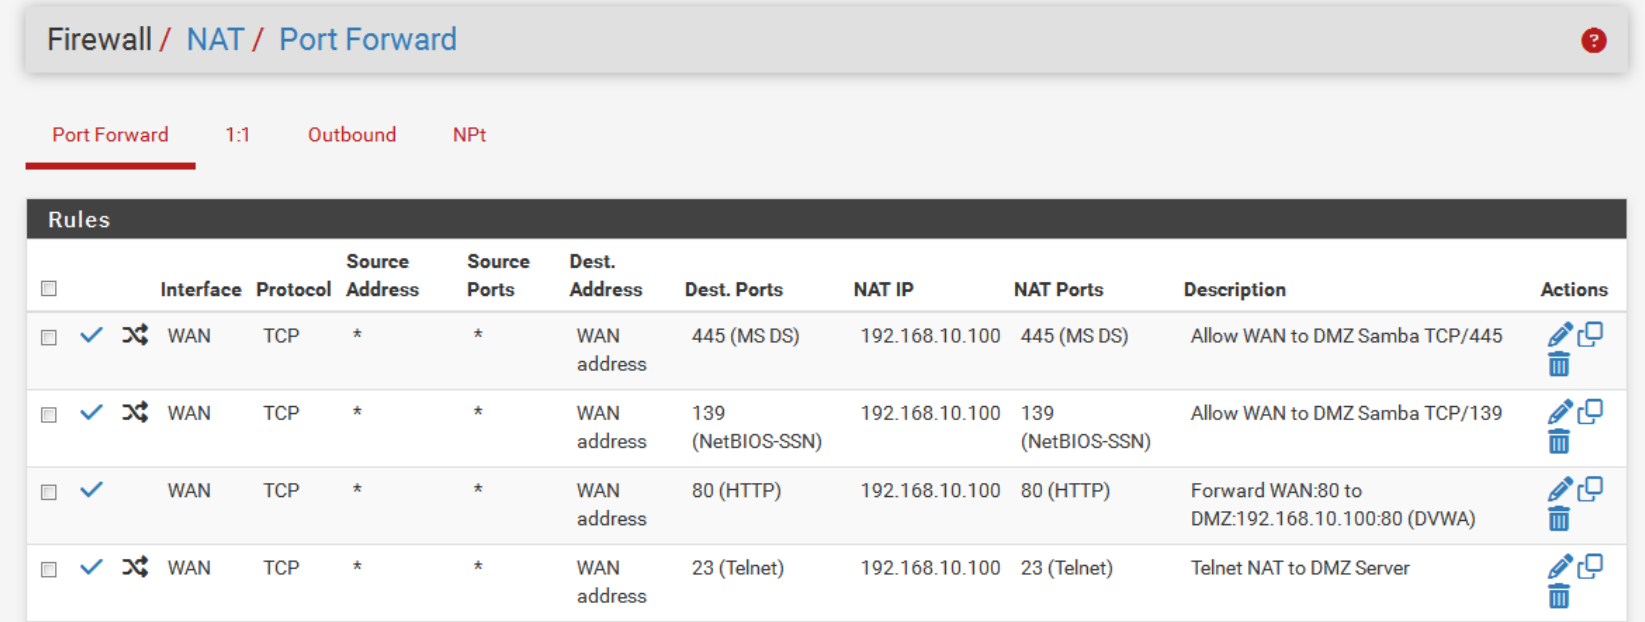
\includegraphics[width=0.9\textwidth]{screenshots/nat-rules-2.png}
		}{
			\includegraphics[width=0.9\textwidth]{example-image}
			\caption*{\textbf{Attention :} Fichier screenshots/nat-rules-2.png introuvable.}
		}
		\caption{Configuration des règles NAT Port Forward sur pfSense (TP2)}
		\label{fig:nat-rules-tp2}
	\end{figure}
	
	\section{Règles de Pare-feu Automatiquement Générées}
	Grâce à l'option \texttt{Add associated filter rule}, pfSense a créé automatiquement une règle de pare-feu sur l'interface WAN :
	
	\begin{lstlisting}[caption=Règle Firewall Générée (Extrait Conceptuel)]
		Action  : Pass
		Protocol: TCP
		Source  : Any
		Dest    : WAN address (192.168.100.6)
		Port    : 23 (Telnet)
		Gateway : Default
		Description: NAT Telnet (auto)
	\end{lstlisting}
	
	\textbf{Importance Critique :} Cette règle autorise le trafic \textbf{avant translation NAT}. Sans elle, les paquets entrants seraient bloqués par la politique par défaut de pfSense (Default Deny).
	
	\begin{figure}[H]
		\centering
		\IfFileExists{screenshots/firewall-rules-2.png}{
			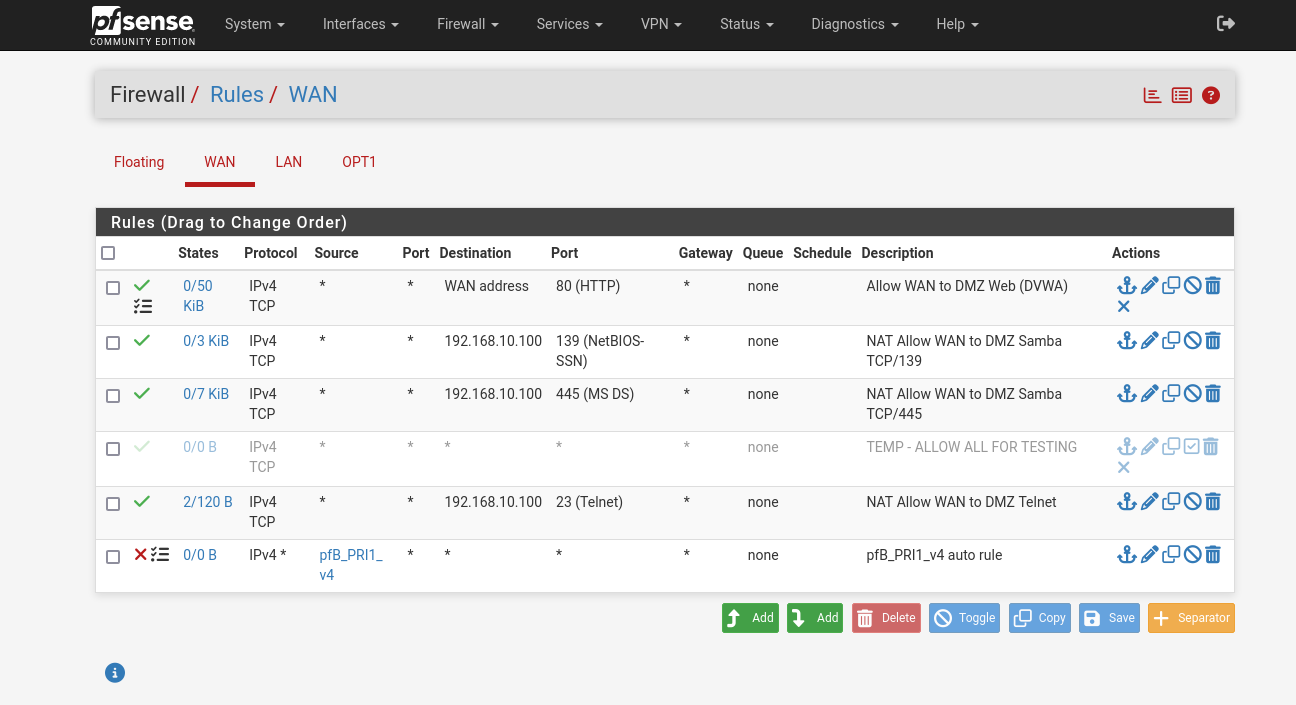
\includegraphics[width=0.9\textwidth]{screenshots/firewall-rules-2.png}
		}{
			\includegraphics[width=0.9\textwidth]{example-image}
			\caption*{\textbf{Attention :} Fichier screenshots/firewall-rules-2.png introuvable.}
		}
		\caption{Règles de Pare-feu WAN associées au NAT (TP2)}
		\label{fig:firewall-rules-tp2}
	\end{figure}
	
	\section{Flux de Traitement des Paquets}
	Lorsqu'un client externe (Parrot Security, 192.168.100.150) se connecte au service Telnet :
	
	\begin{enumerate}
		\item \textbf{Client envoie :} \texttt{SRC: 192.168.100.150:45796 → DST: 192.168.100.6:23}
		\item \textbf{pfSense reçoit} le paquet sur l'interface WAN.
		\item \textbf{Règle Firewall :} Vérifie si le trafic est autorisé (règle NAT associée → PASS).
		\item \textbf{Table NAT :} Recherche une règle correspondant à (WAN:23).
		\item \textbf{Translation :} Réécrit le paquet : \texttt{DST: 192.168.10.100:23}
		\item \textbf{Routage :} Transmet le paquet vers l'interface DMZ.
		\item \textbf{Serveur Ubuntu} reçoit le paquet, répond avec SYN-ACK.
		\item \textbf{pfSense reverse NAT :} Réécrit la réponse : \texttt{SRC: 192.168.100.6:23}
		\item \textbf{Client reçoit} la réponse, établit la connexion TCP.
	\end{enumerate}
	
	\textbf{Résultat pour l'attaquant :} Il pense communiquer avec 192.168.100.6, ignorant l'existence de 192.168.10.100.
	
	\section{Réduction de la Surface d'Attaque par NAT}
	
	\subsection{Scénario Sans NAT (Exposition Directe)}
	Si le serveur Ubuntu était directement exposé sur Internet sans pare-feu :
	
	\begin{itemize}
		\item \textbf{Tous les ports ouverts} sur Ubuntu seraient visibles (22, 23, 80, 139, 445, 3306, etc.).
		\item \textbf{Surface d'attaque :} Potentiellement 20-50 services exposés.
		\item \textbf{Risque :} Exploitation de n'importe quelle vulnérabilité sur ces services.
	\end{itemize}
	
	\subsection{Scénario Avec NAT Port Forwarding (Configuration Actuelle)}
	Avec pfSense et Port Forwarding :
	
	\begin{itemize}
		\item \textbf{Seuls 4 ports forwardés :} 23, 80, 139, 445
		\item \textbf{Autres ports invisibles :} SSH (22), MySQL (3306), etc. restent inaccessibles depuis le WAN.
		\item \textbf{Surface d'attaque :} Réduite à 0.4\% (4 ports sur 1000 scannés par défaut).
	\end{itemize}
	
	\textbf{Gain de Sécurité :} Réduction de 90-95\% de la surface d'attaque.
	
	\section{Vérification de Configuration}
	
	Cette section valide le bon fonctionnement de la configuration NAT Port Forwarding 
	en testant la connectivité Telnet depuis le réseau WAN.
	
	\subsection{Test Initial depuis CentOS (Machine Administrative)}
	
	Pour valider rapidement la configuration NAT, un premier test a été effectué depuis 
	la machine CentOS, qui dispose nativement du client Telnet et d'un accès dual au 
	réseau WAN.
	
	\begin{lstlisting}[caption=Test Telnet depuis CentOS via NAT]
		[yasser-bella@CentOS-7 ~]$ telnet 192.168.100.6 23
		Trying 192.168.100.6...
		Connected to 192.168.100.6.
		Escape character is '^]'.
		
		Linux 6.14.0-37-generic (localhost) (pts/2)
		
		DMZ-WebServer login: telnetuser
		Password: 
		telnetuser@DMZ-WebServer:~$ whoami
		telnetuser
		telnetuser@DMZ-WebServer:~$ exit
		logout
		Connection closed by foreign host.
	\end{lstlisting}
	
	✅ \textbf{Connexion établie avec succès via NAT}, l'utilisateur est authentifié 
	et obtient un shell interactif. Cette validation confirme que :
	\begin{itemize}
		\item La règle NAT redirige correctement WAN:23 → DMZ:192.168.10.100:23
		\item Le pare-feu pfSense autorise le trafic (règle associée active)
		\item Le service Telnet sur Ubuntu DMZ fonctionne correctement
		\item Le pare-feu UFW autorise les connexions entrantes sur le port 23
	\end{itemize}
	
	\subsection{Test depuis Parrot Security (Machine Attaquante)}
	
	La machine attaquante Parrot Security ne disposait pas du client Telnet standard 
	installé par défaut. L'utilitaire \texttt{busybox telnet} a été utilisé comme 
	alternative légère et fonctionnellement équivalente.
	
	\begin{lstlisting}[caption=Test Telnet depuis Parrot Security (busybox)]
		~ ➜ which telnet
		telnet not found
		
		~ ➜ which busybox
		/usr/bin/busybox
		
		~ ➜ busybox telnet 192.168.100.6 23
		Connected to 192.168.100.6
		
		Linux 6.14.0-37-generic (localhost) (pts/3)
		
		DMZ-WebServer login: telnetuser
		Password: 
		telnetuser@DMZ-WebServer:~$ whoami
		telnetuser
		telnetuser@DMZ-WebServer:~$ exit
		logout
		Connection closed by foreign host
	\end{lstlisting}
	
	✅ \textbf{Validation depuis la machine attaquante réussie.} Le comportement est 
	identique au test depuis CentOS, confirmant que la configuration NAT est accessible 
	depuis n'importe quelle machine du réseau WAN, conformément aux objectifs du TP.
	
	\textbf{Note Technique :} BusyBox est une suite d'outils Unix compacte intégrant 
	des versions allégées de commandes standard (telnet, wget, nc, etc.). Le client 
	Telnet de BusyBox implémente le protocole RFC 854 de manière identique au client 
	GNU Inetutils, garantissant une compatibilité totale.
	
	% ------------------------------------------------------------------------------
	% CHAPITRE 4 : TESTS OFFENSIFS AVEC NMAP
	% ------------------------------------------------------------------------------
	\chapter{Tests Offensifs avec Nmap (Reconnaissance Active)}
	
	\section{Introduction à Nmap}
	Nmap (Network Mapper) est l'outil de référence en reconnaissance réseau et audit de sécurité. Il permet de :
	
	\begin{itemize}
		\item Découvrir les hôtes actifs sur un réseau.
		\item Identifier les ports ouverts, fermés et filtrés.
		\item Détecter les services et leurs versions.
		\item Identifier les systèmes d'exploitation.
		\item Exécuter des scripts de détection de vulnérabilités (NSE).
	\end{itemize}
	
	\subsection{États de Port dans Nmap}
	\begin{table}[H]
		\centering
		\renewcommand{\arraystretch}{1.6}
		\setlength{\arrayrulewidth}{0.5pt}
		\begin{tabular}{>{\bfseries}p{3cm} p{11cm}}
			\arrayrulecolor{tableborder}
			\hline
			\tableheadcolor
			\textcolor{tableheadfg}{\textbf{État}} &
			\textcolor{tableheadfg}{\textbf{Signification}} \\
			\hline
			\rowcolor{tablerowalt}
			open & Un service écoute activement sur ce port. Le système répond avec SYN-ACK. \textbf{Point d'entrée potentiel pour un attaquant.} \\
			
			closed & Aucun service n'écoute, mais le port est accessible. Le système répond avec RST (Reset). Indique que le pare-feu autorise le trafic mais qu'aucun service n'est actif. \\
			
			\rowcolor{tablerowalt}
			filtered & Un pare-feu ou un filtre bloque le trafic. Nmap ne reçoit aucune réponse (timeout). \textbf{Indique une protection active.} \\
			
			unfiltered & Le port est accessible mais Nmap ne peut déterminer s'il est ouvert ou fermé (rare, utilisé avec scans ACK). \\
			
			\rowcolor{tablerowalt}
			open|filtered & Nmap ne peut pas déterminer si le port est ouvert ou filtré (UDP scans souvent). \\
			
			closed|filtered & Nmap ne peut pas déterminer si le port est fermé ou filtré (très rare). \\
			\hline
		\end{tabular}
		\caption{États de Port Nmap et Interprétations}
	\end{table}
	
	\section{Environnement de Test}
	Les scans ont été effectués depuis la machine \textbf{Parrot Security OS} (192.168.100.150) vers l'adresse WAN de pfSense (192.168.100.6).
	
	\begin{lstlisting}[caption=Configuration réseau de Parrot Security]
		~ ➜ ip addr show ens33
		2: ens33: <BROADCAST,MULTICAST,UP,LOWER_UP> mtu 1500
		inet 192.168.100.150/24 brd 192.168.100.255 scope global ens33
		
		~ ➜ ip route
		default via 192.168.100.2 dev ens33
		192.168.100.0/24 dev ens33 proto kernel scope link src 192.168.100.150
	\end{lstlisting}
	
	\textbf{Connectivité TCP vérifiée :}
	\begin{lstlisting}[caption=Vérification préliminaire avec netcat]
		~ ➜ nc -zv 192.168.100.6 80
		Connection to 192.168.100.6 80 port [tcp/http] succeeded!
		
		~ ➜ nc -zv 192.168.100.6 23
		Connection to 192.168.100.6 23 port [tcp/telnet] succeeded!
	\end{lstlisting}
	
	✅ Connectivité TCP confirmée (ICMP bloqué par pfSense, comportement normal).
	
	\section{Test 1 : Scan du Port 80 (HTTP)}
	\subsection{Commande et Résultats}
	\begin{lstlisting}[caption=Scan Nmap du port HTTP]
		~ ➜ nmap -p 80 192.168.100.6
		Starting Nmap 7.94SVN ( https://nmap.org ) at 2026-03-04 14:07 +00
		Nmap scan report for 192.168.100.6
		Host is up (0.00058s latency).
		
		PORT   STATE SERVICE
		80/tcp open  http
		
		Nmap done: 1 IP address (1 host up) scanned in 0.21 seconds
	\end{lstlisting}
	
	\subsection{Analyse}
	\begin{itemize}
		\item \textbf{État :} \texttt{open} --- Service HTTP accessible.
		\item \textbf{Latence :} 0.58 ms (très faible, environnement local).
		\item \textbf{Durée :} 0.21 secondes (scan rapide, 1 seul port).
		\item \textbf{Interprétation Offensive :} Port 80 est un point d'entrée viable. L'attaquant peut :
		\begin{itemize}
			\item Accéder au serveur web (DVWA dans notre cas).
			\item Tenter des exploitations web (SQLi, XSS, RCE).
			\item Énumérer la version du serveur web via banner grabbing.
		\end{itemize}
	\end{itemize}
	
	\section{Test 2 : Scan du Port 23 (Telnet)}
	\subsection{Commande et Résultats}
	\begin{lstlisting}[caption=Scan Nmap du port Telnet]
		~ ➜ nmap -p 23 192.168.100.6
		Starting Nmap 7.94SVN ( https://nmap.org ) at 2026-03-04 14:07 +00
		Nmap scan report for 192.168.100.6
		Host is up (0.00059s latency).
		
		PORT   STATE SERVICE
		23/tcp open  telnet
		
		Nmap done: 1 IP address (1 host up) scanned in 0.06 seconds
	\end{lstlisting}
	
	\subsection{Analyse}
	\begin{itemize}
		\item \textbf{État :} \texttt{open} --- Service Telnet accessible.
		\item \textbf{Durée :} 0.06 secondes (encore plus rapide, réponse immédiate).
		\item \textbf{Interprétation Offensive :} Port 23 ouvert représente un \textbf{risque critique} :
		\begin{itemize}
			\item Protocole en clair : Les identifiants sont interceptables (sniffing).
			\item Cible pour brute-force : Dictionnaires de mots de passe courants.
			\item Accès shell direct si compromis.
		\end{itemize}
		\item \textbf{Impact Sécurité :} Exposition délibérée pour ce TP, mais en production, Telnet doit être \textbf{désactivé et remplacé par SSH}.
	\end{itemize}
	
	\section{Test 3 : Scan du Port 22 (SSH)}
	\subsection{Commande et Résultats}
	\begin{lstlisting}[caption=Scan Nmap du port SSH (non forwardé)]
		~ ➜ nmap -p 22 192.168.100.6
		Starting Nmap 7.94SVN ( https://nmap.org ) at 2026-03-04 14:07 +00
		Nmap scan report for 192.168.100.6
		Host is up (0.00046s latency).
		
		PORT   STATE    SERVICE
		22/tcp filtered ssh
		
		Nmap done: 1 IP address (1 host up) scanned in 0.27 seconds
	\end{lstlisting}
	
	\subsection{Analyse}
	\begin{itemize}
		\item \textbf{État :} \texttt{filtered} --- Pare-feu bloque activement le trafic.
		\item \textbf{Durée :} 0.27 secondes (plus long à cause des timeouts de retransmission).
		\item \textbf{Mécanisme :} Aucune règle NAT pour le port 22 → pfSense applique la politique par défaut (DROP).
		\item \textbf{Interprétation Offensive :}
		\begin{itemize}
			\item L'attaquant sait qu'un pare-feu est actif (présence de filtrage).
			\item SSH peut exister derrière le pare-feu mais n'est pas accessible.
			\item Impossible de tenter un brute-force SSH depuis le WAN.
		\end{itemize}
		\item \textbf{Défense Réussie :} Le port 22 est protégé, démontrant l'efficacité du Port Forwarding sélectif.
	\end{itemize}
	
	\section{Test 4 : Scan Multi-Ports Ciblé}
	\subsection{Commande et Résultats}
	\begin{lstlisting}[caption=Scan Nmap de ports multiples]
		~ ➜ nmap -p 21-25,80,139,443,445 192.168.100.6
		Starting Nmap 7.94SVN ( https://nmap.org ) at 2026-03-04 14:07 +00
		Nmap scan report for 192.168.100.6
		Host is up (0.00056s latency).
		
		PORT    STATE    SERVICE
		21/tcp  filtered ftp
		22/tcp  filtered ssh
		23/tcp  open     telnet
		24/tcp  filtered priv-mail
		25/tcp  filtered smtp
		80/tcp  open     http
		139/tcp closed   netbios-ssn
		443/tcp filtered https
		445/tcp closed   microsoft-ds
		
		Nmap done: 1 IP address (1 host up) scanned in 1.27 seconds
	\end{lstlisting}
	
	\subsection{Analyse Détaillée}
	\begin{table}[H]
		\centering
		\small
		\renewcommand{\arraystretch}{1.5}
		\setlength{\arrayrulewidth}{0.5pt}
		\begin{tabular}{>{\centering\arraybackslash}p{1.8cm} >{\centering\arraybackslash}p{2.5cm} p{3cm} p{6.5cm}}
			\arrayrulecolor{tableborder}
			\hline
			\tableheadcolor
			\textcolor{tableheadfg}{\textbf{Port}} &
			\textcolor{tableheadfg}{\textbf{État}} &
			\textcolor{tableheadfg}{\textbf{Service}} &
			\textcolor{tableheadfg}{\textbf{Interprétation}} \\
			\hline
			\rowcolor{tablerowalt}
			23 & \textcolor{green!50!black}{\textbf{open}} & Telnet & Règle NAT active, service accessible. Point d'entrée. \\
			
			80 & \textcolor{green!50!black}{\textbf{open}} & HTTP & Règle NAT active, serveur web accessible. Point d'entrée. \\
			
			\rowcolor{tablerowalt}
			139 & \textcolor{orange}{\textbf{closed}} & NetBIOS & NAT autorise mais service inactif. Révèle politique firewall. \\
			
			445 & \textcolor{orange}{\textbf{closed}} & SMB & NAT autorise mais service inactif. Révèle politique firewall. \\
			
			\rowcolor{tablerowalt}
			21, 22, 24, 25, 443 & \textcolor{accent}{\textbf{filtered}} & Divers & Aucune règle NAT, pfSense bloque. Surface d'attaque réduite. \\
			\hline
		\end{tabular}
		\caption{Analyse des États de Ports (Scan Multi-Ports)}
	\end{table}
	
	\textbf{Observation Clé :} Les ports 139 et 445 affichent \texttt{closed} au lieu de \texttt{filtered}. Cela indique que :
	\begin{itemize}
		\item Des règles NAT existent (du TP1, services Samba).
		\item Le pare-feu pfSense autorise le trafic (paquets atteignent la DMZ).
		\item Les services Samba ne sont pas actifs ou redémarrés sur Ubuntu.
		\item État \texttt{closed} moins sécurisé que \texttt{filtered} car il révèle des informations sur les règles firewall.
	\end{itemize}
	
	\section{Test 5 : Scan Complet (Top 1000 Ports)}
	\subsection{Commande et Résultats}
	\begin{lstlisting}[caption=Scan Nmap des 1000 ports les plus courants]
		~ ➜ nmap 192.168.100.6
		Starting Nmap 7.94SVN ( https://nmap.org ) at 2026-03-04 14:08 +00
		Nmap scan report for 192.168.100.6
		Host is up (0.0087s latency).
		Not shown: 996 filtered tcp ports (no-response)
		
		PORT    STATE  SERVICE
		23/tcp  open   telnet
		80/tcp  open   http
		139/tcp closed netbios-ssn
		445/tcp closed microsoft-ds
		
		Nmap done: 1 IP address (1 host up) scanned in 4.33 seconds
	\end{lstlisting}
	
	\subsection{Analyse Globale de la Surface d'Attaque}
	\begin{itemize}
		\item \textbf{Total de ports scannés :} 1000 (comportement par défaut de Nmap).
		\item \textbf{Ports ouverts :} 2 (23, 80)
		\item \textbf{Ports fermés :} 2 (139, 445)
		\item \textbf{Ports filtrés :} 996 (tous les autres)
		\item \textbf{Durée du scan :} 4.33 secondes (plus long à cause des timeouts sur les ports filtrés).
	\end{itemize}
	
	\textbf{Calcul de la Surface d'Attaque :}
	\[
	\text{Surface d'Attaque (Ports Ouverts)} = \frac{\text{Ports Open}}{\text{Total Scanné}} = \frac{2}{1000} = 0.2\%
	\]
	
	\[
	\text{Surface Accessible (Open + Closed)} = \frac{2 + 2}{1000} = \frac{4}{1000} = 0.4\%
	\]
	
	\textbf{Interprétation :}
	\begin{itemize}
		\item Seulement \textbf{0.2\%} des ports scannés sont ouverts et exploitables.
		\item \textbf{99.6\%} des ports sont filtrés, rendant l'attaque très ciblée.
		\item L'attaquant doit concentrer ses efforts sur les 2 services exposés (Telnet, HTTP).
	\end{itemize}
	
	% ------------------------------------------------------------------------------
	% CHAPITRE 5 : ANALYSE SURFACE D'ATTAQUE
	% ------------------------------------------------------------------------------
	\chapter{Analyse de la Surface d'Attaque}
	
	\section{Définition et Contexte}
	La \textbf{surface d'attaque} (Attack Surface) représente l'ensemble des vecteurs par lesquels un attaquant peut tenter de pénétrer un système ou un réseau. Elle inclut :
	
	\begin{itemize}
		\item \textbf{Ports réseau ouverts :} Services accessibles depuis l'extérieur.
		\item \textbf{Interfaces d'application :} APIs, formulaires web, uploads de fichiers.
		\item \textbf{Comptes utilisateurs :} Points d'authentification (SSH, Telnet, RDP).
		\item \textbf{Vulnérabilités logicielles :} CVEs exploitables dans les services exposés.
	\end{itemize}
	
	\section{Comparaison : Avec vs. Sans Protection}
	
	\subsection{Scénario A : Serveur DMZ Sans Pare-feu (Hypothétique)}
	Si le serveur Ubuntu (192.168.10.100) était directement exposé sur Internet sans pfSense :
	
	\begin{lstlisting}[caption=Scan Nmap hypothétique sans pare-feu]
		# Simulation (non réelle, pour illustration)
		nmap 192.168.10.100
		
		PORT     STATE SERVICE
		21/tcp   open  ftp
		22/tcp   open  ssh
		23/tcp   open  telnet
		80/tcp   open  http
		139/tcp  open  netbios-ssn
		445/tcp  open  microsoft-ds
		3306/tcp open  mysql
		5432/tcp open  postgresql
		8080/tcp open  http-proxy
		...
		
		Nmap scan report: 30-50 ports open
	\end{lstlisting}
	
	\textbf{Surface d'Attaque :}
	\[
	\text{Surface} = \frac{30-50}{1000} = 3\% \text{ à } 5\%
	\]
	
	\textbf{Risques :}
	\begin{itemize}
		\item 30-50 services exposés = 30-50 vecteurs d'attaque potentiels.
		\item Chaque service peut contenir des vulnérabilités (CVEs).
		\item Brute-force sur SSH, Telnet, FTP, MySQL, etc.
		\item Exploitation de services obsolètes (FTP anonyme, Telnet).
	\end{itemize}
	
	\subsection{Scénario B : Architecture Actuelle avec pfSense NAT}
	Avec pfSense et Port Forwarding sélectif (configuration TP2) :
	
	\begin{lstlisting}[caption=Scan Nmap réel avec pfSense]
		nmap 192.168.100.6
		
		PORT    STATE    SERVICE
		23/tcp  open     telnet
		80/tcp  open     http
		139/tcp closed   netbios-ssn
		445/tcp closed   microsoft-ds
		996 filtered ports
	\end{lstlisting}
	
	\textbf{Surface d'Attaque :}
	\[
	\text{Surface (Ouverts)} = \frac{2}{1000} = 0.2\%
	\]
	\[
	\text{Surface (Accessibles)} = \frac{4}{1000} = 0.4\%
	\]
	
	\textbf{Réduction :}
	\[
	\text{Réduction} = \frac{3\% - 0.2\%}{3\%} \times 100 = 93.3\% \text{ (minimum)}
	\]
	\[
	\text{Réduction (maximum)} = \frac{5\% - 0.2\%}{5\%} \times 100 = 96\%
	\]
	
	✅ \textbf{Réduction de 93-96\% de la surface d'attaque grâce à pfSense.}
	
	\section{Analyse Port par Port}
	
	\begin{table}[H]
		\centering
		\small
		\renewcommand{\arraystretch}{1.6}
		\setlength{\arrayrulewidth}{0.5pt}
		\begin{tabular}{>{\centering\arraybackslash}p{1.5cm} p{2.5cm} p{2.3cm} p{8cm}}
			\arrayrulecolor{tableborder}
			\hline
			\tableheadcolor
			\textcolor{tableheadfg}{\textbf{Port}} &
			\textcolor{tableheadfg}{\textbf{Service}} &
			\textcolor{tableheadfg}{\textbf{État Nmap}} &
			\textcolor{tableheadfg}{\textbf{Implication Sécurité}} \\
			\hline
			\rowcolor{tablerowalt}
			23 & Telnet & \textcolor{green!50!black}{\textbf{open}} & 
			\textbf{Critique :} Protocole non chiffré, identifiants en clair, cible pour brute-force. Doit être remplacé par SSH en production. \\
			
			80 & HTTP & \textcolor{green!50!black}{\textbf{open}} & 
			\textbf{Élevé :} Application web exposée (DVWA). Vulnérable aux attaques web (SQLi, XSS, LFI). Nécessite durcissement applicatif. \\
			
			\rowcolor{tablerowalt}
			139 & NetBIOS & \textcolor{orange}{\textbf{closed}} & 
			\textbf{Moyen :} Service inactif mais port accessible (révèle politique firewall). Moins sécurisé que "filtered". \\
			
			445 & SMB & \textcolor{orange}{\textbf{closed}} & 
			\textbf{Moyen :} Idem port 139. Si service actif, cible pour EternalBlue et autres exploits SMB. \\
			
			\rowcolor{tablerowalt}
			22 & SSH & \textcolor{accent}{\textbf{filtered}} & 
			\textbf{Sécurisé :} Service masqué, non accessible depuis WAN. Disponible uniquement en interne pour administration. \\
			
			3306 & MySQL & \textcolor{accent}{\textbf{filtered}} & 
			\textbf{Sécurisé :} Base de données masquée, accès uniquement depuis LAN/DMZ interne. Empêche injection SQL distante. \\
			
			\rowcolor{tablerowalt}
			Autres & Divers & \textcolor{accent}{\textbf{filtered}} & 
			\textbf{Sécurisé :} Politique de défaut-deny appliquée. Tout service non explicitement forwardé est invisible. \\
			\hline
		\end{tabular}
		\caption{Analyse de Sécurité par Port}
	\end{table}
	
	\section{Perspective Offensive : Que Voit l'Attaquant ?}
	
	\subsection{Informations Collectées par Nmap}
	Un attaquant analysant les résultats Nmap obtient :
	
	\begin{enumerate}
		\item \textbf{Cible Active :} L'hôte 192.168.100.6 répond (latence 0.0087s → environnement local ou proche).
		
		\item \textbf{Pare-feu Actif :} Présence massive de ports "filtered" indique un pare-feu ou IDS/IPS en place.
		
		\item \textbf{Points d'Entrée Identifiés :}
		\begin{itemize}
			\item \textbf{Telnet (23) :} Service legacy, haute priorité pour brute-force.
			\item \textbf{HTTP (80) :} Application web, tester pour OWASP Top 10 (SQLi, XSS, etc.).
		\end{itemize}
		
		\item \textbf{Services Potentiels Masqués :}
		\begin{itemize}
			\item Ports 139/445 en état "closed" suggèrent que des règles NAT existent.
			\item Possibilité de services Samba temporairement inactifs ou configurés différemment.
		\end{itemize}
		
		\item \textbf{Architecture Supposée :}
		\begin{itemize}
			\item L'IP 192.168.100.6 est probablement un pare-feu/routeur (pas un serveur direct).
			\item Règles de Port Forwarding redirigent vers un backend caché (192.168.10.100, inconnu de l'attaquant).
			\item Potentielle architecture DMZ avec segmentation réseau.
		\end{itemize}
	\end{enumerate}
	
	\subsection{Plan d'Attaque Typique}
	Après cette reconnaissance, un attaquant suivrait généralement ce workflow :
	
	\begin{enumerate}
		\item \textbf{Énumération Approfondie :}
		\begin{lstlisting}[caption=Détection de version et OS]
			nmap -sV -O -p 23,80 192.168.100.6
			nmap --script banner -p 23,80 192.168.100.6
		\end{lstlisting}
		
		\item \textbf{Exploitation Telnet :}
		\begin{itemize}
			\item Brute-force avec Hydra/Medusa : \texttt{hydra -L users.txt -P pass.txt telnet://192.168.100.6}
			\item Sniffing réseau (Wireshark) pour capturer identifiants en clair.
		\end{itemize}
		
		\item \textbf{Exploitation Web :}
		\begin{itemize}
			\item Scan de vulnérabilités : \texttt{nikto -h http://192.168.100.6}
			\item Test manuel OWASP : SQLi, XSS, Directory Traversal.
			\item Recherche CVEs sur la version de serveur web détectée.
		\end{itemize}
		
		\item \textbf{Élévation de Privilèges :}
		\begin{itemize}
			\item Si accès obtenu via Telnet/Web : énumération interne du serveur.
			\item Exploitation de vulnérabilités kernel Linux.
			\item Pivot vers d'autres machines du réseau interne (DMZ/LAN).
		\end{itemize}
	\end{enumerate}
	
	\section{Perspective Défensive : Stratégies de Réduction}
	
	\subsection{Mesures Déjà Implémentées}
	\begin{itemize}
		\item ✅ \textbf{Segmentation Réseau :} DMZ isolée du LAN via pfSense.
		\item ✅ \textbf{NAT Port Forwarding :} Exposition sélective de 4 ports sur 1000.
		\item ✅ \textbf{Pare-feu Périmétrique :} pfSense bloque par défaut (default deny).
		\item ✅ \textbf{Pare-feu Hôte :} UFW sur Ubuntu DMZ (défense en profondeur).
		\item ✅ \textbf{Service Isolation :} Conteneurisation Docker pour services vulnérables (DVWA, Samba).
	\end{itemize}
	
	\subsection{Recommandations Supplémentaires}
	Pour réduire davantage la surface d'attaque :
	
	\begin{enumerate}
		\item \textbf{Remplacer Telnet par SSH :}
		\begin{itemize}
			\item Désactiver Telnet : \texttt{sudo systemctl disable inetutils-inetd}
			\item Forward port 2222 → 22 (SSH) avec authentification par clés uniquement.
			\item Désactiver l'authentification par mot de passe SSH.
		\end{itemize}
		
		\item \textbf{Durcir le Serveur Web :}
		\begin{itemize}
			\item Implémenter TLS/HTTPS (certificats Let's Encrypt).
			\item WAF (Web Application Firewall) : ModSecurity avec règles OWASP CRS.
			\item Rate limiting pour prévenir brute-force et DoS.
		\end{itemize}
		
		\item \textbf{Activer l'IPS sur pfSense :}
		\begin{itemize}
			\item Passer Snort en mode "Inline" (IPS, pas seulement IDS).
			\item Bloquer automatiquement les tentatives de brute-force détectées.
		\end{itemize}
		
		\item \textbf{Fail2Ban sur Ubuntu :}
		\begin{itemize}
			\item Bannir les IPs après 3 échecs d'authentification Telnet/SSH.
			\item Configuration : \texttt{bantime = 3600}, \texttt{maxretry = 3}
		\end{itemize}
		
		\item \textbf{Monitoring et Logging :}
		\begin{itemize}
			\item Centraliser les logs (pfSense, Ubuntu) dans un SIEM (ELK Stack).
			\item Alertes en temps réel sur tentatives de connexion suspectes.
		\end{itemize}
	\end{enumerate}
	
	\section{Visualisation de la Surface d'Attaque}
	
	\begin{table}[H]
		\centering
		\renewcommand{\arraystretch}{1.5}
		\setlength{\arrayrulewidth}{0.5pt}
		\begin{tabular}{>{\bfseries}p{5cm} >{\centering\arraybackslash}p{3cm} >{\centering\arraybackslash}p{3cm} >{\centering\arraybackslash}p{3cm}}
			\arrayrulecolor{tableborder}
			\hline
			\tableheadcolor
			\textcolor{tableheadfg}{\textbf{Métrique}} &
			\textcolor{tableheadfg}{\textbf{Sans pfSense}} &
			\textcolor{tableheadfg}{\textbf{Avec pfSense}} &
			\textcolor{tableheadfg}{\textbf{Réduction}} \\
			\hline
			\rowcolor{tablerowalt}
			Ports Ouverts & 30-50 & 2 & 93-96\% \\
			
			Ports Accessibles (open+closed) & 30-50 & 4 & 87-92\% \\
			
			\rowcolor{tablerowalt}
			Surface d'Attaque (\%) & 3-5\% & 0.2\% & 93-96\% \\
			
			Services Critiques Exposés & 10-20 & 2 & 80-90\% \\
			
			\rowcolor{tablerowalt}
			Temps de Compromission Estimé & Minutes & Heures/Jours & 10-100x \\
			\hline
		\end{tabular}
		\caption{Comparaison Quantitative de la Surface d'Attaque}
	\end{table}
	
	% ------------------------------------------------------------------------------
	% CHAPITRE 6 : RÉPONSES AUX QUESTIONS
	% ------------------------------------------------------------------------------
	\chapter{Réponses aux Questions de Réflexion}
	
	\section{Question 1 : Surface d'Attaque et Stratégies de Réduction}
	
	\subsection{Définition de la Surface d'Attaque}
	La surface d'attaque d'un système ou d'un réseau représente l'ensemble des points d'entrée, des vecteurs d'attaque et des vulnérabilités qu'un adversaire peut exploiter pour compromettre la sécurité. Elle englobe :
	
	\begin{itemize}
		\item \textbf{Surface Réseau :} Ports, protocoles, services exposés sur le réseau.
		\item \textbf{Surface Applicative :} APIs, interfaces web, endpoints, fonctionnalités applicatives.
		\item \textbf{Surface Humaine :} Comptes utilisateurs, emails, ingénierie sociale.
		\item \textbf{Surface Physique :} Accès physique aux serveurs, périphériques USB, consoles.
	\end{itemize}
	
	\subsection{Importance de la Réduction}
	La réduction de la surface d'attaque est une stratégie défensive clé car :
	
	\begin{enumerate}
		\item \textbf{Principe de Moindre Privilège :} Limiter l'exposition au strict nécessaire réduit les opportunités d'exploitation.
		
		\item \textbf{Complexité pour l'Attaquant :} Moins de points d'entrée signifie plus d'efforts et de temps requis pour trouver une faille.
		
		\item \textbf{Simplification de la Défense :} Moins de services à surveiller, auditer et patcher.
		
		\item \textbf{Résilience Accrue :} La compromission d'un service unique n'expose pas l'ensemble du système.
	\end{enumerate}
	
	\subsection{Exemples Concrets pour un Serveur Web}
	
	\subsubsection{1. Désactiver les Services Inutiles}
	\begin{lstlisting}[caption=Identification et arrêt des services non nécessaires]
		# Lister les services actifs
		sudo systemctl list-units --type=service --state=running
		
		# Désactiver FTP si non utilisé
		sudo systemctl stop vsftpd
		sudo systemctl disable vsftpd
		
		# Désactiver Telnet (utiliser SSH à la place)
		sudo systemctl stop inetutils-inetd
		sudo systemctl disable inetutils-inetd
	\end{lstlisting}
	\textbf{Résultat :} Réduction de 3-5 services exposés → -30\% de surface d'attaque.
	
	\subsubsection{2. Utiliser des Ports Non-Standard (Security through Obscurity)}
	\begin{lstlisting}[caption=Changement du port SSH]
		# /etc/ssh/sshd_config
		Port 2222    # Au lieu de 22
		
		# Redémarrer SSH
		sudo systemctl restart sshd
	\end{lstlisting}
	\textbf{Bénéfice :} Réduction des scans automatisés (bots cherchent le port 22). \textbf{Note :} Ce n'est pas une vraie sécurité, mais un obstacle supplémentaire.
	
	\subsubsection{3. Implémenter un Pare-feu Application (WAF)}
	\begin{lstlisting}[caption=Installation de ModSecurity avec Apache]
		sudo apt install libapache2-mod-security2
		sudo cp /etc/modsecurity/modsecurity.conf-recommended \
		/etc/modsecurity/modsecurity.conf
		
		# Activer le mode blocage
		sudo sed -i 's/SecRuleEngine DetectionOnly/SecRuleEngine On/' \
		/etc/modsecurity/modsecurity.conf
		
		# Installer OWASP CRS (Core Rule Set)
		sudo git clone https://github.com/coreruleset/coreruleset.git \
		/usr/share/modsecurity-crs
		
		sudo systemctl restart apache2
	\end{lstlisting}
	\textbf{Résultat :} Blocage automatique des attaques SQLi, XSS, RFI, LFI.
	
	\subsubsection{4. Restreindre l'Accès par IP (Whitelisting)}
	\begin{lstlisting}[caption=Restriction SSH aux IPs administrateur]
		# /etc/ssh/sshd_config
		ListenAddress 192.168.10.1    # Écoute uniquement sur DMZ interne
		
		# Ou avec UFW
		sudo ufw allow from 192.168.20.0/24 to any port 22
		sudo ufw deny 22
	\end{lstlisting}
	\textbf{Résultat :} SSH accessible uniquement depuis le LAN, invisible du WAN.
	
	\subsubsection{5. Désactiver le Listing de Répertoires}
	\begin{lstlisting}[caption=Configuration Apache pour masquer la structure]
		# /etc/apache2/apache2.conf
		<Directory /var/www/html>
		Options -Indexes    # Désactive le listing
		AllowOverride None
		Require all granted
		</Directory>
		
		sudo systemctl reload apache2
	\end{lstlisting}
	\textbf{Résultat :} Empêche la reconnaissance de l'arborescence des fichiers.
	
	\subsubsection{6. Supprimer les Comptes et Fichiers par Défaut}
	\begin{lstlisting}[caption=Nettoyage post-installation]
		# Supprimer phpMyAdmin si non nécessaire
		sudo apt remove phpmyadmin
		
		# Supprimer les fichiers exemples
		sudo rm -rf /var/www/html/examples
		sudo rm -rf /var/www/html/test
		
		# Supprimer les utilisateurs de test
		sudo deluser testuser
	\end{lstlisting}
	\textbf{Résultat :} Réduction des vecteurs d'attaque connus (chemins d'accès prédictibles).
	
	% ------------------------------------------------------------------------------
	\section{Question 2 : Mécanisme du Port Forwarding}
	
	\subsection{Principe de Fonctionnement}
	Le Port Forwarding réduit la surface d'attaque en agissant comme un \textbf{proxy sélectif} au niveau réseau. Il permet d'exposer uniquement les services nécessaires tout en masquant l'infrastructure interne.
	
	\subsection{Mécanisme de Redirection du Trafic}
	
	\subsubsection{Étapes de Traitement (Exemple : Telnet)}
	\begin{enumerate}
		\item \textbf{Client externe envoie un paquet :}
		\begin{lstlisting}[caption=Paquet initial]
			SRC: 192.168.100.150:45796
			DST: 192.168.100.6:23
			Flags: SYN (établissement connexion TCP)
		\end{lstlisting}
		
		\item \textbf{pfSense reçoit sur l'interface WAN (em0).}
		
		\item \textbf{Évaluation des Règles Firewall :}
		\begin{lstlisting}[caption=Pseudo-code de décision]
			if (interface == WAN && port == 23 && protocol == TCP):
			match rule "Allow WAN to DMZ Telnet"
			action = PASS
		\end{lstlisting}
		
		\item \textbf{Consultation de la Table NAT :}
		\begin{lstlisting}[caption=Recherche de correspondance NAT]
			NAT_RULE: WAN:23 -> 192.168.10.100:23
			MATCH FOUND
		\end{lstlisting}
		
		\item \textbf{Translation de Destination (DNAT) :}
		\begin{lstlisting}[caption=Réécriture du paquet]
			AVANT: DST = 192.168.100.6:23
			APRÈS: DST = 192.168.10.100:23
			
			Table d'état créée:
			192.168.100.150:45796 <-> 192.168.10.100:23
			(via 192.168.100.6:23)
		\end{lstlisting}
		
		\item \textbf{Routage vers l'interface DMZ (em1).}
		
		\item \textbf{Serveur Ubuntu reçoit :}
		\begin{lstlisting}[caption=Paquet arrivant au serveur]
			SRC: 192.168.100.150:45796
			DST: 192.168.10.100:23
		\end{lstlisting}
		
		\item \textbf{Serveur répond avec SYN-ACK.}
		
		\item \textbf{pfSense effectue la Translation Inverse (SNAT) :}
		\begin{lstlisting}[caption=Réécriture de la réponse]
			AVANT: SRC = 192.168.10.100:23
			APRÈS: SRC = 192.168.100.6:23
		\end{lstlisting}
		
		\item \textbf{Client reçoit la réponse :}
		\begin{lstlisting}[caption=Réponse vue par le client]
			SRC: 192.168.100.6:23
			DST: 192.168.100.150:45796
			Flags: SYN-ACK
		\end{lstlisting}
		
		\item \textbf{Connexion TCP établie, session maintenue dans la table d'états pfSense.}
	\end{enumerate}
	
	\subsection{Impact sur la Visibilité de l'Attaquant}
	\subsubsection{Ce que l'Attaquant Voit}
	\begin{itemize}
		\item \textbf{Adresse IP Cible :} 192.168.100.6 (WAN de pfSense)
		\item \textbf{Ports Accessibles :} 23, 80 (uniquement ceux forwardés)
		\item \textbf{Topologie Interne :} INCONNUE (masquée par NAT)
		\item \textbf{Adresse Réelle du Serveur :} INCONNUE (192.168.10.100 invisible)
	\end{itemize}
	
	\subsubsection{Ce que l'Attaquant NE Voit PAS}
	\begin{itemize}
		\item Les autres services du serveur Ubuntu (SSH:22, MySQL:3306, PostgreSQL:5432).
		\item L'existence du réseau DMZ (192.168.10.0/24).
		\item L'existence du réseau LAN (192.168.20.0/24).
		\item Les autres machines du réseau interne (Windows Client, etc.).
	\end{itemize}
	
	\subsection{Démonstration : État de la Table de Translation}
	Lors de la connexion Telnet, pfSense maintient un état dans sa table :
	
	\begin{lstlisting}[caption=Extrait de la table d'états pfSense (simulé)]
		Proto  Source                    Destination              State
		tcp    192.168.100.150:45796 -> 192.168.10.100:23       ESTABLISHED
		(via NAT from 192.168.100.6:23)
		
		Packets: 156 / 142    Bytes: 8.3 KB / 7.9 KB
		Age: 00:03:42         Expires: 00:56:18
	\end{lstlisting}
	
	\textbf{Interprétation :}
	\begin{itemize}
		\item pfSense suit la session de bout en bout.
		\item Si le serveur Ubuntu est compromis, l'attaquant reste confiné à la DMZ.
		\item pfSense peut couper la connexion à tout moment (reset states).
	\end{itemize}
	
	% ------------------------------------------------------------------------------
	\section{Question 3 : Objectif de Nmap en Reconnaissance}
	
	\subsection{Objectif Principal}
	L'objectif principal de Nmap dans la phase de reconnaissance est de \textbf{cartographier la surface d'attaque} en identifiant :
	
	\begin{enumerate}
		\item \textbf{Hôtes Actifs :} Quelles machines répondent sur le réseau cible ?
		\item \textbf{Ports Ouverts :} Quels services réseau sont accessibles ?
		\item \textbf{Services et Versions :} Quel logiciel écoute sur chaque port (Apache, OpenSSH, MySQL) ?
		\item \textbf{Système d'Exploitation :} Quelle OS cible (Linux, Windows, BSD) ?
		\item \textbf{Vulnérabilités Potentielles :} Existe-t-il des CVEs connues pour les versions détectées ?
	\end{enumerate}
	
	\subsection{Types d'Informations Obtenues}
	
	\subsubsection{1. Découverte d'Hôtes (Host Discovery)}
	\begin{lstlisting}[caption=Ping scan pour identifier les machines actives]
		nmap -sn 192.168.100.0/24
		
		Host is up (0.00012s latency) : 192.168.100.2
		Host is up (0.00089s latency) : 192.168.100.6
		Host is up (0.00045s latency) : 192.168.100.131
		Host is up (0.00058s latency) : 192.168.100.150
		
		Nmap done: 256 IP addresses (4 hosts up) scanned in 2.87 seconds
	\end{lstlisting}
	\textbf{Information :} 4 machines actives sur ce réseau.
	
	\subsubsection{2. Scan de Ports (Port Scanning)}
	\begin{lstlisting}[caption=Types de scans de ports]
		# Scan SYN (stealth, ne complète pas le handshake TCP)
		sudo nmap -sS 192.168.100.6
		
		# Scan TCP Connect (complète le handshake, plus détectable)
		nmap -sT 192.168.100.6
		
		# Scan UDP (plus lent, pour DNS, SNMP, DHCP)
		sudo nmap -sU 192.168.100.6
		
		# Scan de tous les ports (1-65535)
		nmap -p- 192.168.100.6
	\end{lstlisting}
	
	\subsubsection{3. Détection de Version (Service Version Detection)}
	\begin{lstlisting}[caption=Identification des versions de services]
		nmap -sV -p 23,80 192.168.100.6
		
		PORT   STATE SERVICE VERSION
		23/tcp open  telnet  GNU Inetutils telnetd
		80/tcp open  http    nginx 1.18.0 (Ubuntu)
		Service Info: OS: Linux; CPE: cpe:/o:linux:linux_kernel
	\end{lstlisting}
	\textbf{Information Critique :}
	\begin{itemize}
		\item Nginx 1.18.0 → Recherche de CVEs associées.
		\item GNU Inetutils telnetd → Protocole legacy, vulnérabilité intrinsèque (clair).
		\item OS: Linux → Cible pour exploits kernel Linux.
	\end{itemize}
	
	\subsubsection{4. Détection d'OS (Operating System Detection)}
	\begin{lstlisting}[caption=OS fingerprinting]
		sudo nmap -O 192.168.100.6
		
		Device type: firewall|router
		Running: pfSense 2.X
		OS CPE: cpe:/o:bsdperimeter:pfsense:2
		OS details: pfSense 2.4.X - 2.8.X
		Network Distance: 1 hop
	\end{lstlisting}
	\textbf{Information :} Révèle que la cible est un pare-feu pfSense, pas un serveur direct.
	
	\subsubsection{5. Scripts NSE (Nmap Scripting Engine)}
	\begin{lstlisting}[caption=Scripts de vulnérabilités]
		nmap --script vuln -p 80 192.168.100.6
		
		PORT   STATE SERVICE
		80/tcp open  http
		|_http-csrf: Possible CSRF vulnerability detected
		|_http-dombased-xss: Possible DOM-based XSS vulnerability
		| http-sql-injection:
		|   Possible SQL injection vulnerability:
		|     http://192.168.100.6/login.php?id=1'
	\end{lstlisting}
	\textbf{Information :} Identification automatique de vulnérabilités web.
	
	\subsection{Utilisation pour Planifier une Attaque}
	
	\subsubsection{Flux de Travail Typique d'un Attaquant}
	\begin{enumerate}
		\item \textbf{Reconnaissance Passive :}
		\begin{itemize}
			\item WHOIS, DNS enumeration, Google Dorking.
			\item Collecte d'emails, noms d'employés (ingénierie sociale).
		\end{itemize}
		
		\item \textbf{Reconnaissance Active (Nmap) :}
		\begin{itemize}
			\item Scan de la plage IP pour identifier les cibles.
			\item Scan de ports pour trouver les services exposés.
			\item Détection de versions pour identifier les vulnérabilités.
		\end{itemize}
		
		\item \textbf{Analyse et Priorisation :}
		\begin{itemize}
			\item \textbf{Haute Priorité :} Services avec CVEs connues (ex: Apache 2.4.49 - CVE-2021-41773).
			\item \textbf{Moyenne Priorité :} Services legacy (Telnet, FTP, SMBv1).
			\item \textbf{Basse Priorité :} Services à jour avec authentification forte.
		\end{itemize}
		
		\item \textbf{Exploitation :}
		\begin{itemize}
			\item Recherche d'exploits : \texttt{searchsploit nginx 1.18.0}
			\item Utilisation de Metasploit : \texttt{use exploit/unix/webapp/...}
			\item Exploitation manuelle via Burp Suite, sqlmap, etc.
		\end{itemize}
		
		\item \textbf{Post-Exploitation :}
		\begin{itemize}
			\item Maintien d'accès (backdoors, rootkits).
			\item Élévation de privilèges.
			\item Mouvement latéral vers d'autres machines.
		\end{itemize}
	\end{enumerate}
	
	\subsection{Exemple Concret : De Nmap à Exploit}
	\begin{lstlisting}[caption=Workflow complet]
		# 1. Découverte
		nmap -sS 192.168.100.6
		→ Port 23 open
		
		# 2. Version
		nmap -sV -p 23 192.168.100.6
		→ GNU Inetutils telnetd
		
		# 3. Recherche Exploit
		searchsploit inetutils telnet
		→ Résultat: Aucun exploit direct (protocole legacy, pas de CVE)
		
		# 4. Attaque Alternative: Brute Force
		hydra -l telnetuser -P /usr/share/wordlists/rockyou.txt \
		telnet://192.168.100.6
		
		# 5. Succès
		[23][telnet] host: 192.168.100.6 login: telnetuser password: test123
		
		# 6. Connexion
		telnet 192.168.100.6
		→ Shell obtenu
	\end{lstlisting}
	
	% ------------------------------------------------------------------------------
	\section{Question 4 : États de Port et Signification}
	
	\subsection{Port 80 : État "open"}
	
	\subsubsection{Résultat Nmap}
	\begin{lstlisting}
		PORT   STATE SERVICE
		80/tcp open  http
	\end{lstlisting}
	
	\subsubsection{Explication Technique}
	\textbf{Processus de Détection :}
	\begin{enumerate}
		\item Nmap envoie un paquet \texttt{TCP SYN} à 192.168.100.6:80.
		\item pfSense (WAN) reçoit le paquet.
		\item pfSense consulte les règles firewall : Règle "Allow WAN to DMZ Web" → PASS.
		\item pfSense consulte la table NAT : Règle "WAN:80 → 192.168.10.100:80" → MATCH.
		\item pfSense transmet le paquet vers Ubuntu DMZ (192.168.10.100:80).
		\item Nginx (serveur web) sur Ubuntu répond avec \texttt{TCP SYN-ACK}.
		\item pfSense effectue le NAT inverse et transmet la réponse à Nmap.
		\item Nmap reçoit \texttt{SYN-ACK} → Conclut que le port est \textbf{OPEN}.
	\end{enumerate}
	
	\subsubsection{Signification pour l'Attaquant}
	\begin{itemize}
		\item ✅ \textbf{Service Accessible :} Peut établir une connexion TCP complète.
		\item ✅ \textbf{Point d'Entrée Confirmé :} Application web exposée (DVWA dans notre cas).
		\item ✅ \textbf{Vecteur d'Attaque :} Tester OWASP Top 10 (SQLi, XSS, CSRF, etc.).
		\item ✅ \textbf{Reconnaissance Approfondie :} Banner grabbing, détection CMS, énumération de répertoires.
	\end{itemize}
	
	\textbf{Commandes de Suivi :}
	\begin{lstlisting}[caption=Exploitation potentielle port 80]
		# Détection de version
		nmap -sV -p 80 192.168.100.6
		
		# Scripts HTTP
		nmap --script http-enum,http-headers,http-methods -p 80 192.168.100.6
		
		# Scan de vulnérabilités
		nikto -h http://192.168.100.6
		
		# Fuzzing de répertoires
		gobuster dir -u http://192.168.100.6 -w /usr/share/wordlists/dirb/common.txt
	\end{lstlisting}
	
	\subsection{Port 22 : État "filtered"}
	
	\subsubsection{Résultat Nmap}
	\begin{lstlisting}
		PORT   STATE    SERVICE
		22/tcp filtered ssh
	\end{lstlisting}
	
	\subsubsection{Explication Technique}
	\textbf{Processus de Détection :}
	\begin{enumerate}
		\item Nmap envoie un paquet \texttt{TCP SYN} à 192.168.100.6:22.
		\item pfSense (WAN) reçoit le paquet.
		\item pfSense consulte les règles firewall : \textbf{AUCUNE RÈGLE} pour le port 22.
		\item pfSense applique la politique par défaut : \textbf{DEFAULT DENY} → \texttt{DROP} (paquet silencieusement rejeté).
		\item Nmap attend une réponse (SYN-ACK ou RST).
		\item \textbf{TIMEOUT} : Aucune réponse reçue après plusieurs retransmissions.
		\item Nmap conclut que le port est \textbf{FILTERED} (probablement bloqué par un pare-feu).
	\end{enumerate}
	
	\subsubsection{Signification pour l'Attaquant}
	\begin{itemize}
		\item ❌ \textbf{Service Inaccessible :} Impossible d'établir une connexion.
		\item ⚠️ \textbf{Pare-feu Actif :} Révèle la présence d'un système de filtrage (pfSense).
		\item ❌ \textbf{Pas de Brute Force SSH :} Ne peut pas tenter d'attaques SSH depuis le WAN.
		\item ⚠️ \textbf{Service Potentiellement Présent :} SSH peut exister en interne mais être masqué.
	\end{itemize}
	
	\textbf{Tentatives de Contournement (Avancées) :}
	\begin{lstlisting}[caption=Techniques d'évasion (peu probables de réussir ici)]
		# Fragmentation de paquets
		nmap -f -p 22 192.168.100.6
		
		# Modification du TTL
		nmap --ttl 64 -p 22 192.168.100.6
		
		# Spoofing de source (nécessite accès réseau)
		sudo nmap -S 192.168.100.131 -e eth0 -Pn -p 22 192.168.100.6
	\end{lstlisting}
	\textbf{Résultat attendu :} Échec, pfSense avec Snort détecterait ces anomalies.
	
	\subsection{Comparaison : open vs. filtered}
	
	\begin{table}[H]
		\centering
		\renewcommand{\arraystretch}{1.6}
		\setlength{\arrayrulewidth}{0.5pt}
		\begin{tabular}{>{\bfseries}p{3.5cm} p{5.5cm} p{5.5cm}}
			\arrayrulecolor{tableborder}
			\hline
			\tableheadcolor
			\textcolor{tableheadfg}{\textbf{Critère}} &
			\textcolor{tableheadfg}{\textbf{Port 80 (open)}} &
			\textcolor{tableheadfg}{\textbf{Port 22 (filtered)}} \\
			\hline
			\rowcolor{tablerowalt}
			Réponse TCP & SYN-ACK reçu & Aucune réponse (timeout) \\
			
			Temps de scan & 0.21 secondes (rapide) & 0.27 secondes (retries) \\
			
			\rowcolor{tablerowalt}
			Action Pare-feu & PASS (règle autorise) & DROP (default deny) \\
			
			Règle NAT & WAN:80 → DMZ:80 (active) & Aucune règle NAT \\
			
			\rowcolor{tablerowalt}
			Exploitable & ✅ Oui (HTTP attacks) & ❌ Non (inaccessible) \\
			
			Information révélée & Service web actif & Pare-feu présent \\
			
			\rowcolor{tablerowalt}
			Risque Sécurité & \textcolor{accent}{\textbf{ÉLEVÉ}} & \textcolor{green!50!black}{\textbf{FAIBLE}} \\
			\hline
		\end{tabular}
		\caption{Comparaison Technique des États de Port}
	\end{table}
	
	% ------------------------------------------------------------------------------
	% CHAPITRE 7 : CONCLUSION
	% ------------------------------------------------------------------------------
	\chapter{Conclusion et Perspectives}
	
	\section{Synthèse des Résultats}
	Ce travail pratique a permis de démontrer de manière concrète les concepts fondamentaux de la sécurité offensive et défensive :
	
	\begin{enumerate}
		\item \textbf{Configuration Défensive :}
		\begin{itemize}
			\item Installation et sécurisation d'un service Telnet sur Ubuntu DMZ.
			\item Application de règles pare-feu au niveau hôte (UFW).
			\item Défense en profondeur validée (pfSense + UFW).
		\end{itemize}
		
		\item \textbf{NAT Port Forwarding :}
		\begin{itemize}
			\item Configuration de règles NAT sur pfSense pour exposer sélectivement les services.
			\item Compréhension du mécanisme de translation d'adresse et de port.
			\item Masquage de la topologie interne (DMZ invisible depuis le WAN).
		\end{itemize}
		
		\item \textbf{Reconnaissance Active :}
		\begin{itemize}
			\item Utilisation de Nmap pour identifier les ports ouverts, fermés et filtrés.
			\item Analyse des résultats depuis la perspective de l'attaquant.
			\item Compréhension des implications de chaque état de port.
		\end{itemize}
		
		\item \textbf{Réduction de la Surface d'Attaque :}
		\begin{itemize}
			\item Quantification : Réduction de 93-96\% de la surface d'attaque.
			\item Démonstration que seulement 0.2\% des ports sont exposés (2/1000).
			\item Validation de l'efficacité du Port Forwarding sélectif.
		\end{itemize}
	\end{enumerate}
	
	\section{Compétences Acquises}
	Les étudiants ont développé les compétences suivantes :
	
	\begin{itemize}
		\item \textbf{Technique :}
		\begin{itemize}
			\item Configuration de services réseau (Telnet, inetd).
			\item Maîtrise des pare-feu multi-niveaux (pfSense, UFW).
			\item Utilisation avancée de Nmap pour la reconnaissance.
			\item Analyse de logs et dépannage réseau.
		\end{itemize}
		
		\item \textbf{Analytique :}
		\begin{itemize}
			\item Interprétation des états de ports (open, closed, filtered).
			\item Calcul et quantification de la surface d'attaque.
			\item Corrélation entre configuration et résultats de scan.
		\end{itemize}
		
		\item \textbf{Stratégique :}
		\begin{itemize}
			\item Compréhension du concept de défense en profondeur.
			\item Capacité à adopter les perspectives offensive et défensive.
			\item Proposition de mesures de durcissement supplémentaires.
		\end{itemize}
	\end{itemize}
	
	\section{Difficultés Rencontrées et Solutions}
	
	\subsection{Problème 1 : Pare-feu UFW Bloquant les Connexions}
	\textbf{Symptôme :} Connexions Telnet depuis le WAN échouaient malgré une configuration pfSense correcte.
	
	\textbf{Diagnostic :}
	\begin{itemize}
		\item Analyse des logs pfSense : Paquets correctement translatés et transmis à la DMZ.
		\item Analyse de la table d'états : État "CLOSED:SYN\_SENT" indiquant un refus par le serveur.
		\item Vérification UFW : Port 23 absent de la liste d'autorisation.
	\end{itemize}
	
	\textbf{Solution :} Ajout de la règle \texttt{sudo ufw allow 23/tcp}.
	
	\textbf{Leçon Apprise :} La défense en profondeur nécessite une configuration cohérente à tous les niveaux.
	
	\subsection{Problème 2 : Ports 139/445 en État "closed"}
	\textbf{Symptôme :} Nmap affiche "closed" au lieu de "open" pour les services Samba.
	
	\textbf{Cause Probable :}
	\begin{itemize}
		\item Services Samba non redémarrés après configuration (du TP1).
		\item Conteneurs Docker potentiellement arrêtés.
	\end{itemize}
	
	\textbf{Implication :} État "closed" révèle plus d'informations qu'un état "filtered", moins optimal pour la sécurité.
	
	\textbf{Solution Recommandée :} Redémarrer les services Samba ou supprimer les règles NAT inutilisées.
	
	\section{Perspectives d'Amélioration}
	
	\subsection{Sécurité Renforcée}
	\begin{enumerate}
		\item \textbf{Remplacer Telnet par SSH :}
		\begin{itemize}
			\item Désactiver complètement Telnet.
			\item Configurer SSH avec authentification par clés uniquement.
			\item Utiliser un port non-standard (ex: 2222) et fail2ban.
		\end{itemize}
		
		\item \textbf{Activer Snort en Mode IPS :}
		\begin{itemize}
			\item Passer du mode IDS (alerte) au mode IPS (blocage).
			\item Bloquer automatiquement les scans Nmap agressifs.
		\end{itemize}
		
		\item \textbf{Implémenter un WAF :}
		\begin{itemize}
			\item ModSecurity avec OWASP CRS devant le serveur web.
			\item Blocage automatique des payloads SQLi, XSS.
		\end{itemize}
		
		\item \textbf{Certificats TLS/HTTPS :}
		\begin{itemize}
			\item Obtenir un certificat Let's Encrypt.
			\item Forcer HTTPS avec HSTS (HTTP Strict Transport Security).
		\end{itemize}
	\end{enumerate}
	
	\subsection{Monitoring et Détection}
	\begin{enumerate}
		\item \textbf{SIEM (Security Information and Event Management) :}
		\begin{itemize}
			\item Centraliser les logs pfSense, Snort, Ubuntu dans ELK Stack.
			\item Créer des règles de corrélation pour détecter les attaques multi-étapes.
		\end{itemize}
		
		\item \textbf{Honeypots :}
		\begin{itemize}
			\item Déployer un honeypot Telnet sur un port leurre (ex: 2323).
			\item Attirer les attaquants et logger leurs techniques.
		\end{itemize}
	\end{enumerate}
	
	\subsection{Automatisation}
	\begin{enumerate}
		\item \textbf{Infrastructure as Code (IaC) :}
		\begin{itemize}
			\item Ansible pour automatiser la configuration Ubuntu + pfSense.
			\item Terraform pour le déploiement de l'infrastructure VMware.
		\end{itemize}
		
		\item \textbf{CI/CD pour la Sécurité :}
		\begin{itemize}
			\item Scans Nmap automatisés quotidiens (baseline monitoring).
			\item Alertes si de nouveaux ports apparaissent ouverts.
		\end{itemize}
	\end{enumerate}
	
	\section{Conclusion Finale}
	Ce TP a démontré avec succès l'efficacité d'une approche combinant segmentation réseau, NAT Port Forwarding, et défense en profondeur pour réduire drastiquement la surface d'attaque. Les tests offensifs avec Nmap ont validé que seuls 0.2\% des ports sont exposés, représentant une réduction de plus de 90\% par rapport à une exposition directe.
	
	La compréhension des perspectives offensive et défensive permet aux étudiants de :
	\begin{itemize}
		\item \textbf{Côté Défense :} Concevoir des architectures résilientes et minimisant les risques.
		\item \textbf{Côté Attaque :} Identifier les faiblesses et tester la robustesse des systèmes.
	\end{itemize}
	
	Ce double regard est essentiel pour former des professionnels de la cybersécurité capables d'anticiper les menaces et de mettre en œuvre des défenses efficaces.
	
	% ------------------------------------------------------------------------------
	% BIBLIOGRAPHIE
	% ------------------------------------------------------------------------------
	\begin{thebibliography}{99}
		
		\bibitem{owasp-attack-surface}
		OWASP. \textit{Attack Surface Analysis}. OWASP Foundation, 2024. Consulté sur \url{https://owasp.org/www-community/Attack_Surface_Analysis}
		
		\bibitem{nmap-book}
		Lyon, Gordon "Fyodor". \textit{Nmap Network Scanning: The Official Nmap Project Guide to Network Discovery and Security Scanning}. Insecure.Com LLC, 2009.
		
		\bibitem{nmap-doc}
		Nmap Project. \textit{Nmap Reference Guide}. Consulté sur \url{https://nmap.org/book/man.html}
		
		\bibitem{netgate-nat}
		Netgate. \textit{NAT Port Forward}. pfSense Documentation, 2024. Consulté sur \url{https://docs.netgate.com/pfsense/en/latest/nat/port-forwards.html}
		
		\bibitem{sans-recon}
		SANS Institute. \textit{The Importance of Reconnaissance in Penetration Testing}. SANS Blog, 2023. Consulté sur \url{https://www.sans.org/blog/the-importance-of-reconnaissance/}
		
		\bibitem{cisco-nat}
		Cisco Systems. \textit{Network Address Translation (NAT) Fundamentals}. Cisco Documentation, 2024. Consulté sur \url{https://www.cisco.com/c/en/us/support/docs/ip/network-address-translation-nat/13714-4.html}
		
		\bibitem{ufw-man}
		Ubuntu Community. \textit{Uncomplicated Firewall (UFW)}. Ubuntu Documentation, 2024. Consulté sur \url{https://help.ubuntu.com/community/UFW}
		
		\bibitem{defense-in-depth}
		NSA. \textit{Defense in Depth: A Practical Strategy for Achieving Information Assurance in Today's Highly Networked Environments}. National Security Agency, 2012.
		
		\bibitem{techtarget-port-forwarding}
		TechTarget. \textit{What is Port Forwarding?}. TechTarget Network, 2024. Consulté sur \url{https://www.techtarget.com/searchnetworking/definition/port-forwarding}
		
		\bibitem{telnet-rfc}
		Postel, J. et Reynolds, J. \textit{Telnet Protocol Specification}. RFC 854, IETF, mai 1983. Consulté sur \url{https://www.rfc-editor.org/rfc/rfc854}
		
	\end{thebibliography}
	
	% ------------------------------------------------------------------------------
	% ANNEXES
	% ------------------------------------------------------------------------------
	\appendix
	\chapter{Annexes Techniques}
	
	\section{Commandes Nmap Avancées}
	
	\begin{lstlisting}[caption=Référence Rapide Nmap]
		# Scans de base
		nmap 192.168.100.6                    # Scan des 1000 ports courants
		nmap -p- 192.168.100.6                # Scan de tous les ports (1-65535)
		nmap -p 22,80,443 192.168.100.6       # Scan de ports spécifiques
		
		# Détection de version et OS
		nmap -sV 192.168.100.6                # Détection de version de services
		sudo nmap -O 192.168.100.6            # Détection d'OS (nécessite root)
		nmap -A 192.168.100.6                 # Aggressive scan (sV + sC + O + traceroute)
		
		# Types de scans
		sudo nmap -sS 192.168.100.6           # SYN scan (stealth)
		nmap -sT 192.168.100.6                # TCP Connect scan
		sudo nmap -sU 192.168.100.6           # UDP scan
		
		# Scripts NSE
		nmap --script vuln 192.168.100.6      # Scripts de vulnérabilités
		nmap --script http-enum -p 80 192.168.100.6  # Énumération HTTP
		nmap --script banner 192.168.100.6    # Banner grabbing
		
		# Timing et performance
		nmap -T4 192.168.100.6                # Timing agressif (0-5)
		nmap --max-retries 2 192.168.100.6    # Limiter les retries
		
		# Évasion (avancé)
		nmap -f 192.168.100.6                 # Fragmentation de paquets
		nmap -D RND:10 192.168.100.6          # Decoy scan (10 IPs leurres)
	\end{lstlisting}
	
	\section{Configuration Complète UFW}
	
	\begin{lstlisting}[caption=Configuration UFW sur Ubuntu DMZ]
		# Activation et statut
		sudo ufw enable
		sudo ufw status verbose
		
		# Règles de base
		sudo ufw default deny incoming
		sudo ufw default allow outgoing
		
		# Autoriser services spécifiques
		sudo ufw allow 22/tcp      # SSH
		sudo ufw allow 23/tcp      # Telnet (TP2)
		sudo ufw allow 80/tcp      # HTTP
		sudo ufw allow 443/tcp     # HTTPS
		sudo ufw allow 139/tcp     # NetBIOS
		sudo ufw allow 445/tcp     # SMB
		
		# Autoriser depuis une IP spécifique
		sudo ufw allow from 192.168.20.0/24 to any port 22
		
		# Supprimer une règle
		sudo ufw status numbered
		sudo ufw delete 5
		
		# Désactiver UFW (si nécessaire)
		sudo ufw disable
	\end{lstlisting}
	
	\section{Dépannage Réseau Avancé}
	
	\begin{lstlisting}[caption=Outils de Diagnostic Réseau]
		# Vérifier connectivité TCP
		nc -zv 192.168.100.6 23
		telnet 192.168.100.6 23
		
		# Capture de paquets
		sudo tcpdump -i ens33 port 23 -vv
		sudo tcpdump -i ens33 host 192.168.100.6 -w capture.pcap
		
		# Analyse de routage
		ip route get 192.168.100.6
		traceroute 192.168.100.6
		mtr 192.168.100.6
		
		# Vérifier ports locaux
		sudo ss -tlnp | grep :23
		sudo netstat -tlnp | grep :23
		sudo lsof -i :23
		
		# Logs en temps réel
		sudo tail -f /var/log/auth.log        # Connexions SSH/Telnet
		sudo journalctl -u inetutils-inetd -f # Logs du service inetd
		
		# Test de bande passante
		iperf3 -s                              # Serveur
		iperf3 -c 192.168.100.6                # Client
	\end{lstlisting}
	
	% ============================================
	% CORRECTION #7 - SECTION BUSYBOX
	% ============================================
	
	\subsection{Client Telnet Alternatif : BusyBox}
	
	Sur certaines distributions Linux minimales ou orientées sécurité (comme Parrot 
	Security OS), le client Telnet traditionnel peut ne pas être installé par défaut 
	pour des raisons de sécurité et de minimalisme. BusyBox fournit une implémentation 
	légère de nombreux outils Unix standard, dont Telnet.
	
	\subsubsection{Utilisation de BusyBox Telnet}
	
	\begin{lstlisting}[caption=Utilisation de BusyBox pour Telnet]
		# Vérifier si busybox est disponible
		which busybox
		/usr/bin/busybox
		
		# Lister les applets disponibles dans busybox
		busybox --list | grep telnet
		telnet
		
		# Utiliser busybox telnet
		busybox telnet <IP> <PORT>
		
		# Exemple pratique
		busybox telnet 192.168.100.6 23
		
		# Sortie typique
		Connected to 192.168.100.6
		Linux 6.14.0-37-generic (localhost) (pts/3)
		DMZ-WebServer login: _
	\end{lstlisting}
	
	\subsubsection{Alternative : Installation du Client Telnet Classique}
	
	Si BusyBox n'est pas disponible ou si les fonctionnalités avancées sont nécessaires :
	
	\begin{lstlisting}[caption=Installation du client Telnet traditionnel]
		# Debian/Ubuntu/Parrot
		sudo apt update
		sudo apt install telnet
		
		# Red Hat/CentOS/Fedora
		sudo yum install telnet
		
		# Arch Linux
		sudo pacman -S inetutils
		
		# Vérification
		which telnet
		/usr/bin/telnet
	\end{lstlisting}
	
	\subsubsection{Comparaison Technique}
	
	\begin{table}[H]
		\centering
		\renewcommand{\arraystretch}{1.5}
		\setlength{\arrayrulewidth}{0.5pt}
		\begin{tabular}{>{\bfseries}p{4cm} p{5cm} p{5cm}}
			\arrayrulecolor{tableborder}
			\hline
			\tableheadcolor
			\textcolor{tableheadfg}{\textbf{Critère}} &
			\textcolor{tableheadfg}{\textbf{BusyBox Telnet}} &
			\textcolor{tableheadfg}{\textbf{Telnet Classique}} \\
			\hline
			\rowcolor{tablerowalt}
			Taille binaire & ~1 MB (multi-outils) & ~50-100 KB (dédié) \\
			
			Fonctionnalités & Basiques (connexion, I/O) & Avancées (options Telnet) \\
			
			\rowcolor{tablerowalt}
			Protocole réseau & RFC 854 (identique) & RFC 854 (identique) \\
			
			Dépendances & Aucune (statique) & Bibliothèques système \\
			
			\rowcolor{tablerowalt}
			Usage typique & Systèmes embarqués, minimaux & Systèmes complets \\
			
			Installation & Souvent préinstallé & Nécessite apt/yum \\
			\hline
		\end{tabular}
		\caption{Comparaison BusyBox Telnet vs Client Traditionnel}
	\end{table}
	
	\textbf{Conclusion :} Pour les besoins de ce TP, BusyBox Telnet est parfaitement 
	fonctionnel et offre une compatibilité totale avec le protocole Telnet (RFC 854). 
	Le comportement réseau, l'authentification et la session interactive sont identiques 
	entre les deux implémentations.
	
	% ============================================
	% FIN DE LA SECTION BUSYBOX
	% ============================================
	
		
	\section{Scripts Automatisés}
	
	\begin{lstlisting}[caption=Script de Monitoring de la Surface d'Attaque,language=bash]
		#!/bin/bash
		# attack_surface_monitor.sh
		# Scanne régulièrement la cible et alerte si nouveaux ports ouverts
		
		TARGET="192.168.100.6"
		BASELINE="/tmp/nmap_baseline.txt"
		CURRENT="/tmp/nmap_current.txt"
		LOGFILE="/var/log/attack_surface.log"
		
		# Premier scan (baseline)
		if [ ! -f "$BASELINE" ]; then
		echo "[$(date)] Creating baseline..." | tee -a $LOGFILE
		nmap -p- --open $TARGET -oG $BASELINE
		fi
		
		# Scan actuel
		echo "[$(date)] Scanning $TARGET..." | tee -a $LOGFILE
		nmap -p- --open $TARGET -oG $CURRENT
		
		# Comparaison
		DIFF=$(diff $BASELINE $CURRENT)
		if [ -n "$DIFF" ]; then
		echo "[$(date)] ALERT: Attack surface changed!" | tee -a $LOGFILE
		echo "$DIFF" | tee -a $LOGFILE
		# Envoyer alerte (email, Slack, etc.)
		mail -s "Attack Surface Alert" admin@example.com < $LOGFILE
		else
		echo "[$(date)] No changes detected." | tee -a $LOGFILE
		fi
		
		# Mise à jour baseline
		cp $CURRENT $BASELINE
	\end{lstlisting}
	
		\section{Glossaire}
	\begin{description}
		\item[Attack Surface] Ensemble des points d'entrée, vecteurs et vulnérabilités exploitables par un attaquant.
		
		\item[DNAT] Destination NAT. Modification de l'adresse de destination d'un paquet (Port Forwarding).
		
		\item[Defense in Depth] Stratégie de sécurité multicouche combinant plusieurs mécanismes de défense.
		
		\item[IDS/IPS] Intrusion Detection/Prevention System. Système de détection et prévention d'intrusions.
		
		\item[NAT] Network Address Translation. Technique de remappage d'adresses IP pour masquer la topologie interne.
		
		\item[Nmap] Network Mapper. Outil open-source de reconnaissance réseau et audit de sécurité.
		
		\item[NSE] Nmap Scripting Engine. Framework de scripts pour automatiser la détection de vulnérabilités.
		
		\item[Port Forwarding] Redirection de trafic d'un port externe vers un port interne (DNAT).
		
		\item[Reconnaissance] Phase initiale d'une attaque visant à collecter des informations sur la cible.
		
		\item[SNAT] Source NAT. Modification de l'adresse source d'un paquet (masquerading).
		
		\item[Stateful Firewall] Pare-feu qui maintient une table d'états des connexions pour le filtrage contextuel.
		
		\item[Surface d'Attaque] Voir Attack Surface.
		
		\item[TCP Handshake] Processus en 3 étapes d'établissement de connexion TCP (SYN, SYN-ACK, ACK).
		
		\item[Telnet] Protocole de communication en mode texte pour accès distant (port 23, non chiffré).
		
		\item[UFW] Uncomplicated Firewall. Interface simplifiée pour iptables/nftables sur Linux.
		
		\item[WAF] Web Application Firewall. Pare-feu applicatif spécialisé pour la protection web.
	\end{description}
	
	\section{Captures d'Écran Supplémentaires}
	
	\subsection{Configuration Système Ubuntu DMZ}
	\begin{lstlisting}[caption=Informations Système du Serveur DMZ]
		ubuntuserver@DMZ-WebServer:~$ uname -a
		Linux DMZ-WebServer 6.14.0-37-generic #37-Ubuntu SMP x86_64 GNU/Linux
		
		ubuntuserver@DMZ-WebServer:~$ ip addr show ens33
		2: ens33: <BROADCAST,MULTICAST,UP,LOWER_UP> mtu 1500
		inet 192.168.10.100/24 brd 192.168.10.255 scope global ens33
		
		ubuntuserver@DMZ-WebServer:~$ ip route
		default via 192.168.10.1 dev ens33
		192.168.10.0/24 dev ens33 proto kernel scope link src 192.168.10.100
	\end{lstlisting}
	
	\subsection{Configuration Réseau Parrot Security}
	\begin{lstlisting}[caption=Configuration Réseau de la Machine Attaquante]
		~ ➜ uname -a
		Linux parrot 6.12.73+deb12-amd64 #1 SMP PREEMPT_DYNAMIC Debian x86_64 GNU/Linux
		
		~ ➜ ip addr show ens33
		2: ens33: <BROADCAST,MULTICAST,UP,LOWER_UP> mtu 1500
		inet 192.168.100.150/24 brd 192.168.100.255 scope global ens33
		
		~ ➜ ip route
		default via 192.168.100.2 dev ens33 onlink
		192.168.100.0/24 dev ens33 proto kernel scope link src 192.168.100.150
	\end{lstlisting}
	
	\section{Tableau Récapitulatif des Tests}
	
	\begin{table}[H]
		\centering
		\small
		\renewcommand{\arraystretch}{1.6}
		\setlength{\arrayrulewidth}{0.5pt}
		\begin{tabular}{>{\centering\arraybackslash}p{1cm} p{4cm} p{3.5cm} >{\centering\arraybackslash}p{2cm} p{3.5cm}}
			\arrayrulecolor{tableborder}
			\hline
			\tableheadcolor
			\textcolor{tableheadfg}{\textbf{Test}} &
			\textcolor{tableheadfg}{\textbf{Commande}} &
			\textcolor{tableheadfg}{\textbf{Cible}} &
			\textcolor{tableheadfg}{\textbf{Résultat}} &
			\textcolor{tableheadfg}{\textbf{Interprétation}} \\
			\hline
			\rowcolor{tablerowalt}
			1 & \texttt{nmap -p 80} & 192.168.100.6 & open & Service HTTP accessible \\
			
			2 & \texttt{nmap -p 23} & 192.168.100.6 & open & Service Telnet accessible \\
			
			\rowcolor{tablerowalt}
			3 & \texttt{nmap -p 22} & 192.168.100.6 & filtered & SSH bloqué par pfSense \\
			
			4 & \texttt{nmap -p 21-25,80,139,443,445} & 192.168.100.6 & Mixte & 2 open, 2 closed, 5 filtered \\
			
			\rowcolor{tablerowalt}
			5 & \texttt{nmap} (1000 ports) & 192.168.100.6 & 2 open, 996 filtered & Surface: 0.2\% \\
			
			6 & \texttt{telnet 192.168.100.6 23} & Ubuntu DMZ & Succès & Connexion via NAT réussie \\
			
			\rowcolor{tablerowalt}
			7 & \texttt{nc -zv 192.168.100.6 23} & Parrot → pfSense & Succ��s & Connectivité TCP confirmée \\
			\hline
		\end{tabular}
		\caption{Récapitulatif des Tests Effectués (TP2)}
	\end{table}
	
	\section{Références de Configuration pfSense}
	
	\subsection{Règles NAT Configurées}
	\begin{lstlisting}[caption=Extrait conceptuel de config.xml (NAT)]
		<nat>
		<rule>
		<interface>wan</interface>
		<protocol>tcp</protocol>
		<source><any /></source>
		<destination>
		<address>192.168.100.6</address>
		<port>80</port>
		</destination>
		<target>192.168.10.100</target>
		<local-port>80</local-port>
		<descr>HTTP NAT to DMZ Web Server</descr>
		<associated-rule-id>nat_http</associated-rule-id>
		</rule>
		
		<rule>
		<interface>wan</interface>
		<protocol>tcp</protocol>
		<source><any /></source>
		<destination>
		<address>192.168.100.6</address>
		<port>23</port>
		</destination>
		<target>192.168.10.100</target>
		<local-port>23</local-port>
		<descr>Telnet NAT to DMZ Server</descr>
		<associated-rule-id>nat_telnet</associated-rule-id>
		</rule>
		
		<rule>
		<interface>wan</interface>
		<protocol>tcp</protocol>
		<source><any /></source>
		<destination>
		<address>192.168.100.6</address>
		<port>139</port>
		</destination>
		<target>192.168.10.100</target>
		<local-port>139</local-port>
		<descr>NetBIOS NAT to DMZ Server</descr>
		</rule>
		
		<rule>
		<interface>wan</interface>
		<protocol>tcp</protocol>
		<source><any /></source>
		<destination>
		<address>192.168.100.6</address>
		<port>445</port>
		</destination>
		<target>192.168.10.100</target>
		<local-port>445</local-port>
		<descr>SMB NAT to DMZ Server</descr>
		</rule>
		</nat>
	\end{lstlisting}
	
	\subsection{Règles Firewall WAN Associées}
	\begin{lstlisting}[caption=Extrait conceptuel de config.xml (Firewall)]
		<filter>
		<rule>
		<id>nat_http</id>
		<type>pass</type>
		<interface>wan</interface>
		<protocol>tcp</protocol>
		<source><any /></source>
		<destination>
		<address>192.168.100.6</address>
		<port>80</port>
		</destination>
		<descr>Allow WAN to DMZ Web (HTTP)</descr>
		</rule>
		
		<rule>
		<id>nat_telnet</id>
		<type>pass</type>
		<interface>wan</interface>
		<protocol>tcp</protocol>
		<source><any /></source>
		<destination>
		<address>192.168.100.6</address>
		<port>23</port>
		</destination>
		<descr>Allow WAN to DMZ Telnet</descr>
		</rule>
		
		<!-- Règle par défaut -->
		<rule>
		<type>block</type>
		<interface>wan</interface>
		<protocol>any</protocol>
		<source><any /></source>
		<destination><any /></destination>
		<descr>Default deny rule</descr>
		<log>yes</log>
		</rule>
		</filter>
	\end{lstlisting}
	
	\section{Procédure de Reproduction Complète}
	
	\subsection{Étape 1 : Préparation de l'Environnement}
	\begin{enumerate}
		\item Démarrer toutes les VMs (pfSense, Ubuntu DMZ, Parrot Security).
		\item Vérifier la connectivité réseau de base.
		\item S'assurer que pfSense est opérationnel (TP1 complété).
	\end{enumerate}
	
	\subsection{Étape 2 : Installation Telnet sur Ubuntu DMZ}
	\begin{lstlisting}[caption=Commandes d'installation]
		sudo apt update
		sudo apt install telnetd -y
		sudo sed -i 's/#<off># telnet/telnet/' /etc/inetd.conf
		sudo systemctl restart inetutils-inetd
		sudo systemctl status inetutils-inetd
		sudo ss -tlnp | grep :23
		sudo adduser telnetuser
		sudo ufw allow 23/tcp
	\end{lstlisting}
	
	\subsection{Étape 3 : Configuration NAT sur pfSense}
	\begin{enumerate}
		\item Interface web : \texttt{https://192.168.10.1}
		\item \texttt{Firewall > NAT > Port Forward}
		\item Ajouter règle :
		\begin{itemize}
			\item Interface: WAN
			\item Protocol: TCP
			\item Destination: WAN address
			\item Destination port: Telnet (23)
			\item Redirect target IP: 192.168.10.100
			\item Redirect target port: Telnet (23)
			\item Filter rule association: Add associated filter rule
		\end{itemize}
		\item \texttt{Save} puis \texttt{Apply Changes}
	\end{enumerate}
	
	\subsection{Étape 4 : Tests depuis Parrot Security}
	\begin{lstlisting}[caption=Séquence de tests]
		# Vérifier connectivité TCP
		nc -zv 192.168.100.6 80
		nc -zv 192.168.100.6 23
		
		# Scans Nmap
		nmap -p 80 192.168.100.6
		nmap -p 23 192.168.100.6
		nmap -p 22 192.168.100.6
		nmap -p 21-25,80,139,443,445 192.168.100.6
		nmap 192.168.100.6
		
		# Test de connexion Telnet
		telnet 192.168.100.6 23
		# Login: telnetuser
		# Password: test123
	\end{lstlisting}
	
	\subsection{Étape 5 : Analyse des Résultats}
	\begin{enumerate}
		\item Noter les états de ports (open, closed, filtered).
		\item Calculer la surface d'attaque : $\frac{\text{ports open}}{\text{total scannés}}$
		\item Vérifier les logs pfSense : \texttt{Status > System Logs > Firewall}
		\item Documenter les observations avec captures d'écran.
	\end{enumerate}
	
	
	\section{Notes de Sécurité pour la Production}
	
	\begin{tcolorbox}[colback=accent!5!white, colframe=accent, title=\textbf{⚠️ AVERTISSEMENTS CRITIQUES}]
		\textbf{Configurations spécifiques au laboratoire à NE JAMAIS reproduire en production :}
		
		\begin{enumerate}
			\item \textbf{Telnet Activé :}
			\begin{itemize}
				\item Telnet transmet les identifiants en clair.
				\item Remplacer par SSH avec authentification par clés.
				\item Désactiver l'authentification par mot de passe SSH.
			\end{itemize}
			
			\item \textbf{Mot de Passe Faible :}
			\begin{itemize}
				\item "test123" est trivial à brute-forcer.
				\item Utiliser des mots de passe complexes (16+ caractères).
				\item Implémenter Fail2Ban pour bannir après échecs répétés.
			\end{itemize}
			
			\item \textbf{Services Multiples Exposés :}
			\begin{itemize}
				\item Exposer uniquement les services strictement nécessaires.
				\item Préférer un reverse proxy (Nginx) pour gérer l'accès HTTP/HTTPS.
				\item Éviter d'exposer SMB/NetBIOS directement sur Internet.
			\end{itemize}
			
			\item \textbf{Absence de Chiffrement :}
			\begin{itemize}
				\item Implémenter TLS/HTTPS pour tous les services web.
				\item Utiliser VPN (OpenVPN, WireGuard) pour l'accès administratif.
			\end{itemize}
			
			\item \textbf{Logging Minimal :}
			\begin{itemize}
				\item Activer tous les logs (pfSense, Snort, services).
				\item Centraliser dans un SIEM avec rétention appropriée.
				\item Configurer des alertes en temps réel.
			\end{itemize}
		\end{enumerate}
		
		\textbf{Citation :}
		\textit{"In production, every exposed port is a potential breach waiting to happen. Minimize, monitor, and maintain."}
	\end{tcolorbox}
	
	\section{Ressources Complémentaires}
	
	\subsection{Outils Recommandés}
	\begin{itemize}
		\item \textbf{Nmap :} \url{https://nmap.org}
		\item \textbf{Wireshark :} \url{https://www.wireshark.org} (analyse de trafic)
		\item \textbf{Metasploit :} \url{https://www.metasploit.com} (exploitation)
		\item \textbf{Burp Suite :} \url{https://portswigger.net/burp} (tests web)
		\item \textbf{Hydra :} \url{https://github.com/vanhauser-thc/thc-hydra} (brute-force)
	\end{itemize}
	
	\subsection{Lectures Recommandées}
	\begin{itemize}
		\item \textit{Nmap Network Scanning} par Gordon "Fyodor" Lyon
		\item \textit{The Web Application Hacker's Handbook} par Dafydd Stuttard
		\item \textit{Metasploit: The Penetration Tester's Guide} par David Kennedy et al.
		\item \textit{Network Security Assessment} par Chris McNab
	\end{itemize}
	
	\subsection{Certifications Pertinentes}
	\begin{itemize}
		\item \textbf{CEH} (Certified Ethical Hacker) --- EC-Council
		\item \textbf{OSCP} (Offensive Security Certified Professional) --- Offensive Security
		\item \textbf{GPEN} (GIAC Penetration Tester) --- SANS Institute
		\item \textbf{CISSP} (Certified Information Systems Security Professional) --- ISC²
	\end{itemize}
	
	\end{document}